% !TEX root = ../thesis_main.tex
%
%
%
%%%% --- * --- %%%%	
\clearpage
%\chapter{Atomic Physics Overview}
%\chapter{General Considerations of Atomic Techniques Used}
\chapter{Considerations and Implementation of Atomic Techniques}
\label{atomicphysics_chapter}

%\note[color=jb]{JB:  First, I'm pretty sure you should combine Chs. 3 and 4 (now 2 and 3) (( now just Ch.2)). 
%Ch 4 (3) has good solid general description and details in situ about optical
%pumping and about the photoionization probe that are, unfortunately, wrong in Ch. 3(2).
%You could call the first half of such a chapter "General considerations of Atomic techniques used"
%and the 2nd half "Experimental Implementation of Atomic Techniques used"}
%\note[color=todoblue]{wtf could I possibly have gotten wrong in my Ch.3 description?  It's so vague!}

\note{Possible Supersection:  General Considerations of Atomic Techniques Used}
\section{An Overview of Magneto-Optical Traps}
\note[color=org]{I need to organize the sections/subsections in this chapter better...}
Since its initial description by Raab et. al. in 1987~\cite{raabprentiss}, the magneto-optical trap (MOT) has become a widely used technique in many atomic physics laboratories.  The MOT produces confined samples of cold, electrically neutral and isotopically pure atoms confined within a small spatial region.  It is these properties that make the MOT a valuable tool not only in atomic physics, but for precision measurements in nuclear physics as well, and the TRINAT lab \aside[color=org]{Have I defined TRINAT yet?} has adopted the technique wholeheartedly.

The technique is used predominantly with alkalis due to their simple orbital electron structure,% so is appropriate for use with $^{37}\textrm{K}$.  
and once set up it is quite robust.  The MOT's trapping force is specific to the isotope for which the trap has been tuned. This feature makes it ideal for use in precision radioactive decay experiments, since the daughters are unaffected by the trapping forces keeping the parent confined.
\note[color=org]{Possibly most of the above paragraph is also written/paraphrased elsewhere.  Like in ((Ch.2B)), unless I removed it...}
%\note{... used predominantly with alkalis due to their simple orbital electron structure.}

A typical MOT can be created from relatively simple components:  a quadrupole-shaped magnetic field, typically generated by two current-carrying coils of wire, and a circularly polarized laser tuned to match one or more atomic transitions in the isotope of interest.  Because a MOT is easily disrupted by interactions with untrapped atoms, the trap must be created within a vaccuum system.  Finally, a source of atoms to be trapped is required.  [See Fig.~\ref{fig:mot}.]

%There are two primary components necessary for any MOT:  a laser, and a magnetic field.  
The laser, which must be circularly polarized in the appropriate directions and tuned slightly to the red of an atomic resonance, is split into three perpendicular retroreflected beams, doppler cooling the atoms and (with the appropriate magnetic field) confining them in all three dimensions (see Figure~\ref{fig:mot}).  
%The TRINAT science chamber includes 6 `viewports' specifically designed to be used for the trapping laser.


\note{``In order to understand the mechanism by which a MOT is able to confine atoms, we must first introduce the Zeeman effect (Section 2.1) and a description of an optical molasses (Section 2.2). A functional MOT combines the forces resulting from these two mechanisms to trap and cool atoms.''}

%The TRINAT lab has adopted this technique from atomic physics to perform nuclear physics experiments.  
%Such samples may subsequently be used in a variety of physical measurements.
%\note{``Since the magneto-optical trap (MOT) was first described in 1987 by Raab et. al.~\cite{raabprentiss}, it has become a standard technique for confining cold samples of neutral atoms.  These cold trapped atoms may subsequently be used in the measurement of a variety of physical quantities."}


\subsection{Zeeman Splitting}
In the presence of an external magnetic field $\vec{B}$, the Hamiltonian associated with an atom's orbital electrons will acquire an additional ``Zeeman Shift'' term, given by~\cite{corney}
\bea
\label{zeeman_hamiltonian}
H_{\mathrm{\,Zeeman}} &=& - \vec{\mu}\cdot \vec{B},
\eea
where $\vec{\mu}$ is the magnetic moment associated with the orbital under consideration.  In the limit where the magnetic field is too weak to significantly disrupt the coupling between the electron's spin- and orbital angular momenta, $\vec{\mu}$ may be treated as being fixed with respect to changes in the magnetic field.  It is this weak field regime which will be primarily of interest to us in work with magneto-optical traps.


With $\vec{\mu}$ fixed, it is clear that the magnitude of the energy shift must scale linearly with the strength of the magnetic field.  In considering the perturbation to the energy of a particular \emph{transition}, the perturbations to the initial and final states must of course be subtracted:
\bea
\Delta E_{\mathrm{\,transition}} &=& - \left( \vec{\mu}_f - \vec{\mu}_i \right) \cdot \vec{B}.
\eea 



%an atom's orbital energy levels take on a perturbation.  The perturbation to the Hamiltonian is given by
%
%the energy levels associated with an atom's electron orbitals are perturbed.  

%\note{Needs work.}
%\note{Needs an equation.}
\note{Needs a level diagram.  Maybe.}

%The Zeeman shift is what happens when you stick an atom in a magnetic field.  An atom's energy levels, which would have been degenerate before applying a field, split according the angular momentum.  At low fields (which is what is of interest to us here), the energy perturbation scales linearly with the strength of the magnetic field.  

\note{
When this is combined with a circularly polarized laser beam, the effect is to move the atomic resonance closer to- or farther from- the frequency of the laser.  The circular polarization, combined with some selection rules, means a circularly polarized laser will only couple to one particular transition, w.r.t. angular momentum.  ie, for a $\sigma_+$ polarized laser, the atom's overall angular momentum projection (along some axis) will be incremented by $+1$.  The Zeeman shift means that in a magnetic field, this transition (M+=1) not be the same as the M-=1 transition.  So, if you have a magnetic field that changes linearly across space, you can make it so that in $+ B_z$ regions, the laser beam with one certain polarization is closer to resonance and therefore more likely to be absorbed -- and similarly, in $- B_z$ regions, a different laser with the opposite polarization will be more likely to be absorbed.  Again, if the B-field is linear in space, you can do it so that as the atoms get further and further from the `centre' region, the effect gets progressively stronger.  So, if you've done this right, you can make it so that the atoms get a stronger ``push'' back towards the center the farther away they've drifted.
\\
They still get the optical molasses cooling effect for free.}


\subsection{Saturation Spectroscopy}
\note[color=jb]{JB says:  Chapter 3 (that's this chapter) ((Now Ch.2A)):
Starting in Ch. 3 around p. 10, "Atom-Photon Interactions with a Laser" (that's this section -- now ``Saturation Spectroscopy''):
\\
You need to do a careful pass through it and omit everything you don't understand and don't need.
\\
Sorry, there is no longer time to resolve your questions unless you need them.}

\note{This is a stupid subsection title.}
%We consider first the interaction between a single atom and a single photon.  Suppose 

Consider a single two-level atom in its ground state interacting with a single photon with the same energy as that of a the atomic transition between the ground and excited states.  If angular momentum selection rules allow it\aside{Also, if the photon is tuned close enough to atomic resonance, with absorption being more likely the smaller the detuning is...}, the photon will be absorbed and the atom will receive a ``push'' 
from the incident 
%
%proportional to the 
%detuning\aside{Wait.  I don't think I got that right.  Detuning only affects absorption probability, right?  I guess it also has an effect on the size of the push, but that's really not the primary pushing effect going on here.} of the photon from the atomic resonance.  
%
photon's momentum.  
After a time, the atom will spontaneously de-excite by emitting a photon in a random direction.  Conservation of momentum results in the atom receiving a second push from the emitted photon.  

If one considers a cloud of many such atoms within the path of a correctly-tuned (low intensity) laser beam, then provided the atoms are constrained to remain within the beam path, the result of many such interactions is a biased random walk in physical space for each individual atom, and a net velocity change for the cloud as a whole.
% such that the cloud as a whole receives a change in net velocity. 

In contrast to the above description of absorption followed by spontaneous emission, a photon interacting with an atom in the excited state may cause the atom to de-excite by emitting a second photon.  This mechanism is negligible in the case of a sufficiently low intensity laser beam.  However, as the laser intensity increases, so too will the fraction of atoms in the excited state at any given time.  As it is only the excited state atoms that are able undergo stimulated emission, this effect becomes increasingly dominant as the intensity of the incident laser increases.  In the limit of infinite intensity, stimulated emission and absorption are equally likely to occur, and therefore the population is split evenly between the ground and excited states.  

To describe the regime change between atomic interactions with low intensity- and high intensity lasers, we introduce the (on-resonance) saturation intensity, $I_{\mathrm{sat}}$, where 
\bea
I_{\mathrm{sat}} &=& \frac{\hbar \omega_0^3 \gamma}{12\pi c^2}
\eea
is the laser intensity at which the rates of decay by stimulated- and spontaneous emission are equal, $\hbar \omega_0$ is the energy of both the atomic transition %and also an individual photon, 
and $\gamma$ describes the linewidth of the atomic transition and equivalently its rate of spontaneous decay from its excited state.  We may further define the on-resonance saturation parameter $s_0$, for a laser of intensity $I$ as,
\bea
s_0 &:=& \frac{I}{ I_{\mathrm{sat}} }.
\eea

In practice, for the project that is the topic of this thesis, the MOT laser operates at about 1/2 of saturation intensity, while the optical pumping
and photoionization lasers operate at considerably lower than saturation
intensity. However, one can gain
%most lasers operate in the high intensity regime -- the obvious exception being the photoionization laser (see Section whatever)
%\aside[color=org]{Where have I even decided to put the photoionization section, anyway?}  
%However, one can still gain 
a qualitative understanding of many aspects of atom-laser interaction while neglecting saturation concerns.  
\note[color=done]{Fixed description of which lasers are saturated.}
%\aside{Clunky phrasing.} 
%\aside[color=todoblue]{Do I need saturation to make an optical molasses?  I bet I do.}  
\note{Do I need to mention saturation at all?  It's probably not really necessary, and I don't *think* anything else in this section is wrong per se.  But maybe better to just cut it.}

%\note[color=jb]{JB says:  "In practice, for the project that is the topic of this thesis,
%most lasers operate in the high intensity regime –
%the obvious exception being the photoionization laser (see Section whatever)
%However, one can still gain ..."
%\\
%change to ->
%\\
%"In practice, for the project that is the topic of this thesis,
%the MOT laser operates at about 1/2 of saturation intensity,
%while the optical pumping
%and photoionization lasers operate at considerably lower than saturation
%intensity.
%However, one can gain ..."}
%
% % % 

\subsection{Doppler Cooling}
% % % 
We now consider a somewhat more general case in which a cloud of two-level atoms lies along the path of two counter-propagating laser beams, both detuned slightly to the red of resonance.  For simplicity, this cloud will be treated as being constrained in the other two dimensions such that it must within the laser's path.  With two counter-propagating laser beams of equal intensity and detuning,\aside{...and opposite polarization.  Or something.  I have to talk about the selection rules somewhere else.} the ``push'' from interaction with one beam is exactly counteracted by the push from the opposite-propagating beam, and there is no net velocity transfer to the cloud.  

Detuning the laser from resonance will of course decrease absorption upon interacting with an atom at rest -- however the atoms within the cloud are not at rest, but rather are undergoing thermal motion.  As such, within the rest frame of each individual atom, the two laser beams will appear to be Doppler shifted in opposite directions, with the sign dependent on atomic motion.  In particular, atoms moving against a laser's direction of propagation will see that laser beam as being blueshifted.  Since the laser has been red-detuned within the lab frame, the blueshift moves the laser frequency as seen by the atom back toward resonance, and makes its photons more likely to be absorbed.  Similarly, for an atom moving in the same direction as a red-detuned laser beam, this laser will be seen as further red-shifted, and absorption likelihood is decreased.  Because of the difference in absorption, such an atom becomes more likely to receive a push back against its (lab frame) direction of motion, slowing it down, and less likely to recieve a push to increase its lab frame speed.   \aside{Optical molasses equation?  Maybe?}

The overall effect on a one-dimensional cloud of atoms in the path of two counter-propagating red-detuned lasers is that the atoms will be slowed and cooled.  Such a setup is sometimes referred to as a one-dimensional ``optical molasses'' due to the viscous drag force induced on atomic motion.  It is straightforward to extend this model to three dimensions.  Although this setup will decrease atomic velocity, it does not include a confining force, so the atoms are still free to move out of the lasers' path, albeit at a decreased speed.  


%The laser's red detuning with respect to the atomic resonance 

%being used are of a sufficiently high intensity  
%\note{``Such a setup is sometimes referred to as a one-dimensional “optical molasses” due to the viscous drag force induced on atomic motion, which will be discussed in more detail shortly.''}
%\note{``In such a system, an incident photon can excite an atom from the ground state into the excited state, while simultaneously giving the atom a “push” proportional to the laser’s detuning from the atomic resonance.''}

%Consider an atom in one dimension in the midst of two counter-propagating laser beams which are otherwise identical.   ...Ugh.
\note{``...This will slow the atom down, at least up to a limit related to the linewidth of the atomic transition and/or the laser.  There's something to look up.''}
%\note{Needs an equation. (?)}
%\note{Needs work.}
%\note[color=org]{I should really split these things back up into subsections.  Zeeman shift, saturation intensity, optical molasses/doppler cooling.  Then selection rules.}

%First, consider an atom in an optical molasses.  in 1D, that means there are two counter-propogating lasers, both tuned slightly to the red of an atomic transition.  Also, they're polarized s.t. ... something.  The point is, atoms moving against the direction of a red-detuned laser's propagation will see a doppler shifted laser frequency, tuned closer to the atomic transition, which makes a photon more likely to be absorbed.  Similarly, the opposite-propagating laser will appear to be further red-shifted away from resonance.  When a photon is absorbed, we require conservation of (linear) momentum, so the atom gets a ``push'' against the direction it was travelling.  This will slow the atom down, at least up to a limit related to the linewidth of the atomic transition and/or the laser.  There's something to look up.
%
%Anyway, when you have two counter-propagating red-detuned lasers, the net effect will be to slow the atom's motion down a bunch.  It's called an optical molasses, because the photons are sticky or whatever.  By itself, it does not confine atoms, it only slows them down.

%%%% % % % %%%
%\subsection{Angular Momentum and Selection Rules}
%\note[color=jb]{JB:  3.1.4 Angular Momentum and Selection Rules (that's this section!):
%\\
%Sorry, this section is almost entirely wrong, and you don't need it.
%Omit it please.}
%
%\note[color=jb]{JB:  Agreed it's ok to ignore the repumper laser.}
%
%As in any other interaction, when a photon and an atom interact with one another, angular momentum must be conserved.
%%In any interaction, angular momentum must be conserved, and the interactions between atoms and photons are no exception.  
%An individual photon has spin 1, and therefore when we consider an atom-photon interaction where the photon is absorbed, the atom's total angular momentum projection \comment{(I think on any axis???)} must also change by one unit.
%\note{Fuck.  What even *are* the other rules?  Have to change F too?  I think that's true.. Clearly I have to look this up.}
%On a macroscopic level, the polarization of a laser can be used as a stand-in to describe, in a probabilistic way, the spin orientation of the individual photons of which the beam consists.  
%
%\note{I mean.  I probably don't need to go too in-depth here.  But I haven't mentioned it at all yet, and it's a relevant thing.}
%Polarization matters.  You have to conserve angular momentum.  In fact, you have to conserve both total angular momentum *and* its projection on whatever axis.  Photons have spin-1, but because they literally go at the speed of light, they can't do $0 \rightarrow 0$ transitions.  
%
%This is related to why you need repumpers for your MOT, but also, I don't really want to get into that.  But also-also, why even *would* you?  You don't in the description I've already given.  Pretty sure it's because you can sometimes de-excite to a *stupid* set of energy levels.  And then, I don't think they really fall back down or something?  I've largely forgotten how it works.  Ugh.
\note[color=done]{Removed `Angular Momentum and Selection Rules' section.  Because it was super wrong.}

%%% % % % %%%
\subsection{Atom Trapping with a MOT}
\note[color=jb]{JB:  on 3.3 (now 2.3) ``Atom Trapping with a MOT''  ((that's here!)):
\\
The content and scope are ok, but the informal phrasing is going to
confuse people. You have to pay some attention and rephrase these sections. }

\note{Do I *have* an equation I can put here?  Surely there must be one somewhere, but I really don't want to dig it up, and I don't think it's really necessary.}
\note{Needs work.}
Really, at the end of the previous section, I described the MOT's trapping mechanism.  That's literally what it is.  You just need to do it in 3 dimensions, rather than only one.  Fortunately, an anti-helmholz(sp?) coil gives us a quadrupole-shaped magnetic field, which *actually* has a magnetic field that changes linearly along any axis in the region near the center.   

Optical molasses + zeeman splitting = magneto-optical trap.  Anyway, see Fig.~\ref{fig:mot}.

\note{Do I *really* need to bring up the repumper?  I don't wanna.  Maybe I can just mention it and move on or something.}

\begin{figure}[h!!!!!t!]
	\centering
		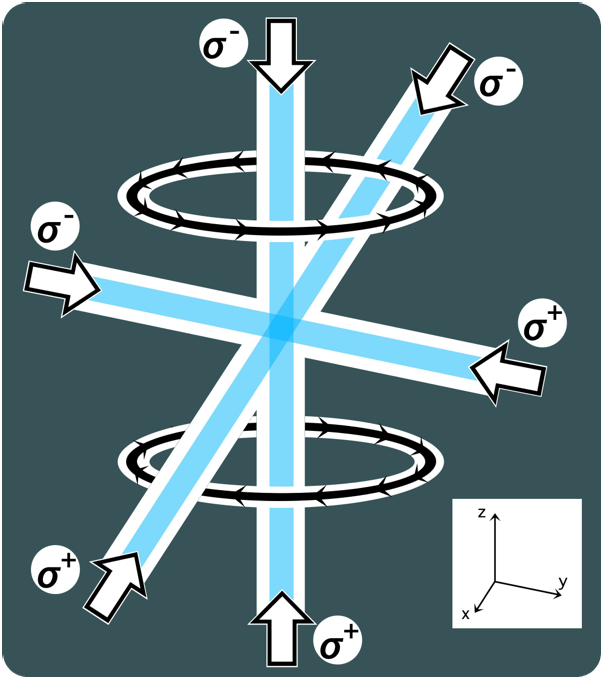
\includegraphics[width=.999\linewidth]{mot.png}
		\caption{Components of a magneto-optical trap, including current-carrying magnetic field coils and counterpropagating circularly polarized laser beams. Diagram taken from~\cite{thesis}}
		\label{fig:mot}
    	\label{fig:themot}
\end{figure}



\note[color=done]{Removed `Photoionization as a Probe' section from the `Intro to Atomic Physics' section, because John says it's horribly wrong anyhow.  Plus, it's redundant with the `Photoionization Laser' section~(\ref{photoions}).}
%\section{Photoionization as a Probe}
%\label{sec:photoprobe}
%\note[color=jb]{JB on 3.5 `Photoionization as a probe' (that's this section!):
%\\
%You describe this well in 4.4 "Photoionization laser"
%\\
%So I recommend strongly you cut  the whole 3.5 section,
%because it's incomplete, and what you
%have contains errors.
%\\ ... \\
%Here are things there are not time to understand:
%\\ ... \\
%about 1/3 of the MOT atoms are excited, not 'a large fraction'
%\\ ... \\
%yes, we've intentionally polarized the OP laser to be circular so the
%atoms will be polarized. We've also picked the S 1/2 to P1/2 so that the
%fully stretched S1/2 $F=2$ $m_F=2$ state is dark. (Unlike the MOT, where we
%need the P3/2 state so that atoms never go dark,  or the force would stop.)
%But we agreed above not to talk about this.
%\\ ... \\
%"We have a photodiode(?) to observe what fraction of things get photoionized overall."
%\\ ... \\
%no, we look at the photoionization rate, for which we have the ion vs. photodiode TOF (`photodiode' looks at when the bursts of light occur)
%}
%
%So, the photoionization laser.  It ionizes only $\approx 1\%$ of the atoms, so it's mostly non-destructive.  
%
%For atoms in a MOT, it can give a projection of the trap position.  At least, it can if you add some MCPs with delay lines, and an electric field.  Also, the atoms have to be excited or they don't get photoionized this way.  That's because at any given time, a large fraction of the trapped atoms are in the excited state, so it works.
%
%For polarized or partially polarized atoms, absorption stops, because of selection rules.  We've intentionally polarized the laser to do this.  I think.  \aside[color=todoblue]{*Have* we even polarized the photoionization laser in any particular way?  I'm not sure we even have.  Why doesn't it absorb?  When it's stretched, it's not just all in the excited state!  It's...stretched.  Do angular momentum selection rules even apply if the electron is going into the continuum?}
%
%\note{Include a picture of the trap.  Possibly on both the rMCP and the eMCP.  Also, maybe a thing for the polarization as a function of time?  But I don't really need to do that, because it's in the paper.}
%
%Anyway, the probing only works if you have a detector to see what things.  We have a photodiode(?) to observe what fraction of things get photoionized overall.  This gives us polarization.  We also have an MCP with delay lines, and an electric field to guide (positive) ions into it.  And another MCP with delay lines on the other side of the electric field, to collect the electrons removed by photoionization.  Also, the (orbital) electrons removed during beta decay.  The photoionization laser is pulsed.  So, when there's a pulse, we can check whether there was a hit detected in the ion detector and/or the electron detector.  It turns out, we can't check both at the same time, because our two detectors hate each other.  They're natural enemies, really.  Turns out, the ion detector is better at measuring the polarization, and the trap position.  Because reasons.  \aside[color=org]{But it's worse for $\Abeta$ and $\bFierz$, because .... reasons that probably shouldn't go in this chapter.}  Anyway, during the 2014 run, we spent like half of the beamtime collecting ions and half collecting electrons.  \aside[color=org]{This also doesn't go in this section.}


%%% % % % %%%
\section{Optical Pumping}
\label{sec:op}
\note[color=jb]{Direct quote from John follows below:  }
\comment{The optical pumping process is described in detail in our collaboration’s Ref.~\cite{ben_OP}. The main detail described here is that the optical pumping is distrubed by any component of magnetic field not along the quantization axis. (Ours is the vertical axis, defined by the direction of the optical pumping light, and along which the detectors are placed.) This required sophistication with an AC MOT described below.}

\note[color=jb]{End quote from John.  But also!:
\\
``...Then you can refer to that (ie, John's red quoted mini-blurb about optical pumping, (which I may relocate to Sec.~\ref{photoions}?  Or not?) in section 3.4 (now 2.4, about the AC-MOT -- ie, Sec.~\ref{sec:acmot}, (even though I might remove that section entirely and put all its content into Sec.~\ref{section:acmot_and_polarization}) ), where you're trying to now but the phrasing is poor.''}

%\note{Needs work.}
\note{``Until recently, one limitation of such samples was the necessity for the presence of a relatively large magnetic field, which is expected to partially destroy atomic polarization, limiting the precision of many types of measurements.  Here we discuss the construction of a newer type of MOT, the AC-MOT, which minimizes residual magnetic fields.  The guys in~\cite{harveymurray} came up with the idea of the AC-MOT.  They made it work and did some stuff with it.  Good for them.''}
Need a nice, uniform, constant magnetic field for your polarization to larmor precess around.  Then, however depolarized (from the axis of the magnetic field) you were to start out, you don't like precess in a way that changes the projection you care about.

But also, I should actually describe the optical pumping, too.  And point at Ben's OP paper that we did~\cite{ben_OP}.

\note[color=org]{Somewhere later, I can talk about photoionization?  Or should it be here, in this chapter?  Surely it should at least get a different section though.}

%\missingfigure{I need \emph{at least} one atomic level diagram.  But possibly as many as 3 level diagrams.  Have to show energies for MOT, energies for OP, and energies for photoionization.  }

%\note{Needs a better level diagram.  Or possibly no level diagrams at all.}
%\note{Previous assertion:  I need \emph{at least} one atomic level diagram.  But possibly as many as 3 level diagrams.  Have to show energies for MOT, energies for OP, and energies for photoionization.}
\note{Do I need a MOT level diagram too?}

\begin{figure}[h!!t]
	\centering
	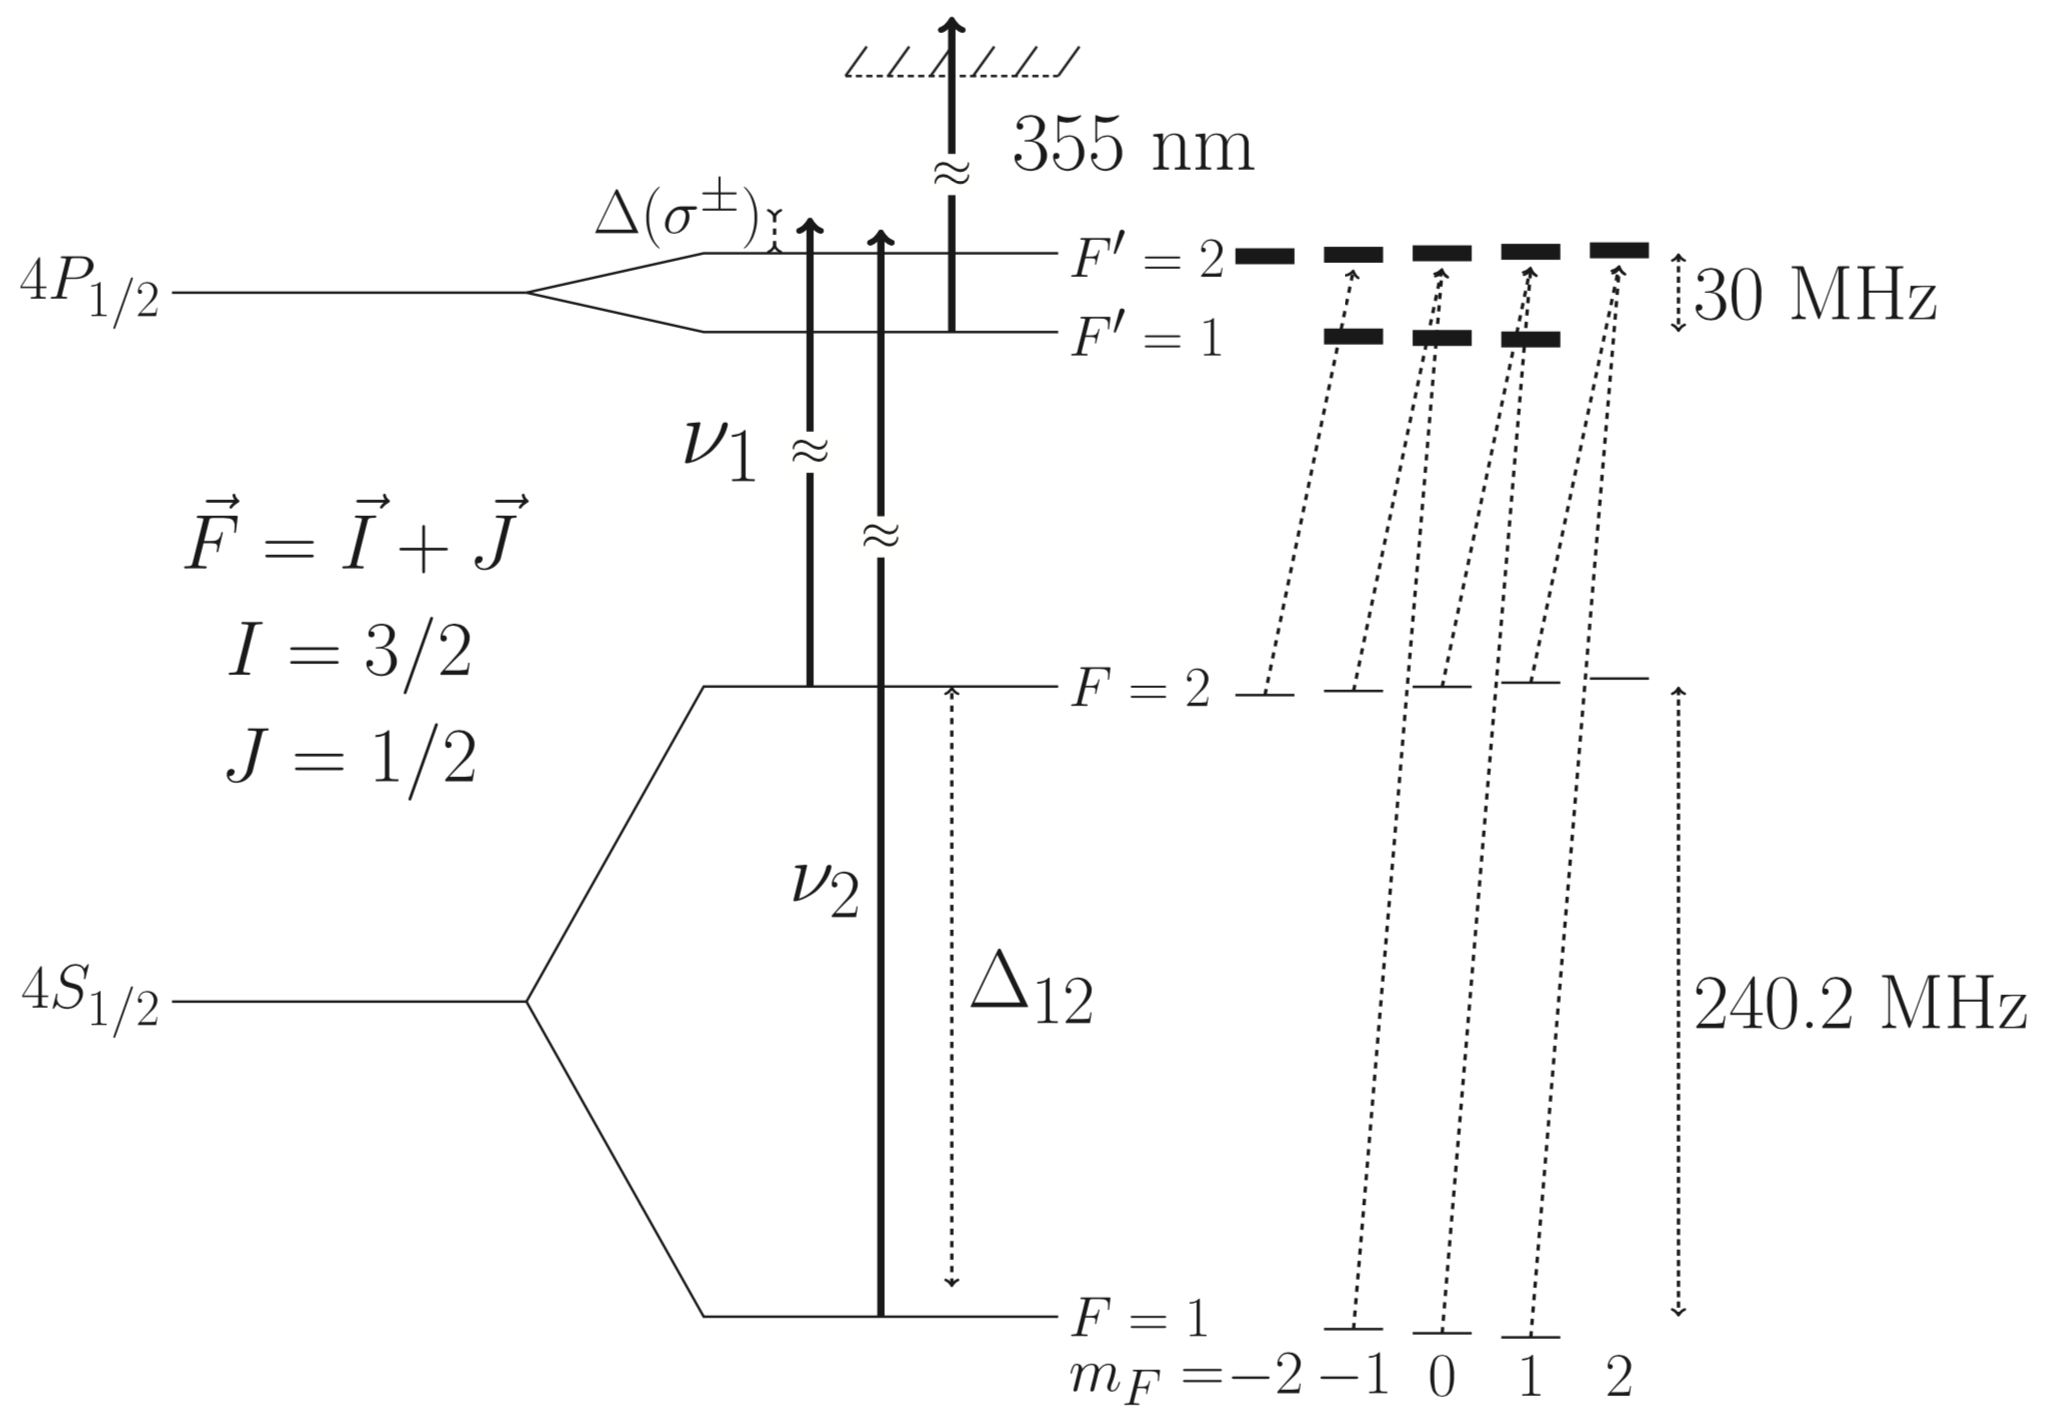
\includegraphics[width=.999\linewidth]
	{Figures/OP_LevelDiagram_bf.png}
	\note{Describe what's going on here!}
	\caption{An atomic level diagram for the optical pumping of $\isotope[37]{K}$, taken from \cite{ben_OP}.  }	
	\label{fig:op_leveldiagram}
\end{figure}

\note[color=purple]{JB says:  ``I would say you don't need an atomic level diagram.  You could just describe in words the semiclassical picture of atoms absorbing photons until they are nearly fully polarized, then they stop absorbing.  The optical pumping + photoionization is then an in situ probe of the polarization. ... You would need to add in words that quantum mechanical corrections to this picture are in the optical Bloch equation approach in B. Fenker et al.  The depolarized states still have high nuclear polarization (1/2 for $F=2, M_F=1$, 5/6 for $F=1, M_F=1$) and determining the ratio of those two populations provides most of the info we need -- we model with the O.B.E, measure the optical pumping light polarization, and float an average transverse magnetic field.  This is adequate to determine the depolarized fraction to 10\% accuracy, which is all that is needed.'' }








% !TEX root = ../thesis_main.tex
% 
% 
% 
% 
%%%% --- * --- %%%%	
%\clearpage
\section{An Overview of the Double MOT System and Duty Cycle}
\label{section:overview}
%\chapter{The Experimental Setup}
%\chapter{Experimental Implementation}
\label{experimental_chapter}
\label{setup_chapter}

%\note[color=done]{JB:  First, I'm pretty sure you should combine Chs. 3 and 4 (now 2 and 3) (( now just Ch.2)).  Ch 4 (3) ((2B)) has good solid general description and details in situ about optical pumping and about the photoionization probe that are, unfortunately, wrong in Ch. 3(2)((2A)).}
\note[color=jb]{JB:  
%First, I'm pretty sure you should combine Chs. 3 and 4 (now 2 and 3) (( now just Ch.2)).  Ch 4 (3) ((2B)) has good solid general description and details in situ about optical pumping and about the photoionization probe that are, unfortunately, wrong in Ch. 3(2)((2A)).
...You could call the first half of such a chapter "General considerations of Atomic techniques used" and the 2nd half "Experimental Implementation of Atomic Techniques used"}

\note{Supersection:  Experimental Implementation of Atomic Techniques Used}

\note{Remember the pulser LED!  To evaluate the stability of the scintillator gain!}

\note[color=done]{JB says:  chapter (((this section))) is really good, and in good shape for the committee}

\note{
We obtain a sample of neutral, cold, nuclear spin-polarized $^{37}\textrm{K}$ atoms with a known spatial position, via the TRIUMF accelerator facility, by intermittently running a magneto-optical trap (MOT) to confine and cool the atoms, then cycling the trap off to polarize the atoms.  With $\beta$ detectors placed opposite each other along the axis of polarization, we are able to directly observe the momenta of $\beta^+$ particles emitted into 1.4\% of the total solid angle nearest this axis.  We also are able to extract a great deal of information about the momentum of the recoiling $^{37\!}$Ar daughters by measuring their times of flight and hit positions on a microchannel plate detector with a delay line.  Because the nuclear polarization is known to within $<0.1\%$~\cite{ben_OP}, and we are able to account for many systematic effects by periodically reversing the polarization and by collecting unpolarized decay data while the atoms are trapped within the MOT, we expect to be well equipped to implement a test of `handedness' within the nuclear weak force.
}


The experimental subject matter of this thesis was conducted at TRIUMF using the apparatus of the TRIUMF Neutral Atom Trap (TRINAT) collaboration.  The TRINAT laboratory offers an experimental set-up which is uniquely suited to precision tests of Standard Model beta decay physics, by virtue of its ability to produce highly localized samples of cold, isotopically pure atoms within an open detector geometry.  \aside[color=org]{Surely most of this paragraph goes in an intro chapter somewhere.}  Although the discussion in this chapter will focus on the methodologies used to collect one particular dataset, taken over approximately 7 days of beamtime in June 2014, the full apparatus and the techniques used are fairly versatile, and can be (and have been) applied to
several related experiments using other isotopes.
\note{Cite a bunch of papers here.}
%\note{mumble mumble 7ish days of beamtime, mumble mumble 2014.}

\begin{figure}[t!h]
	\centering
	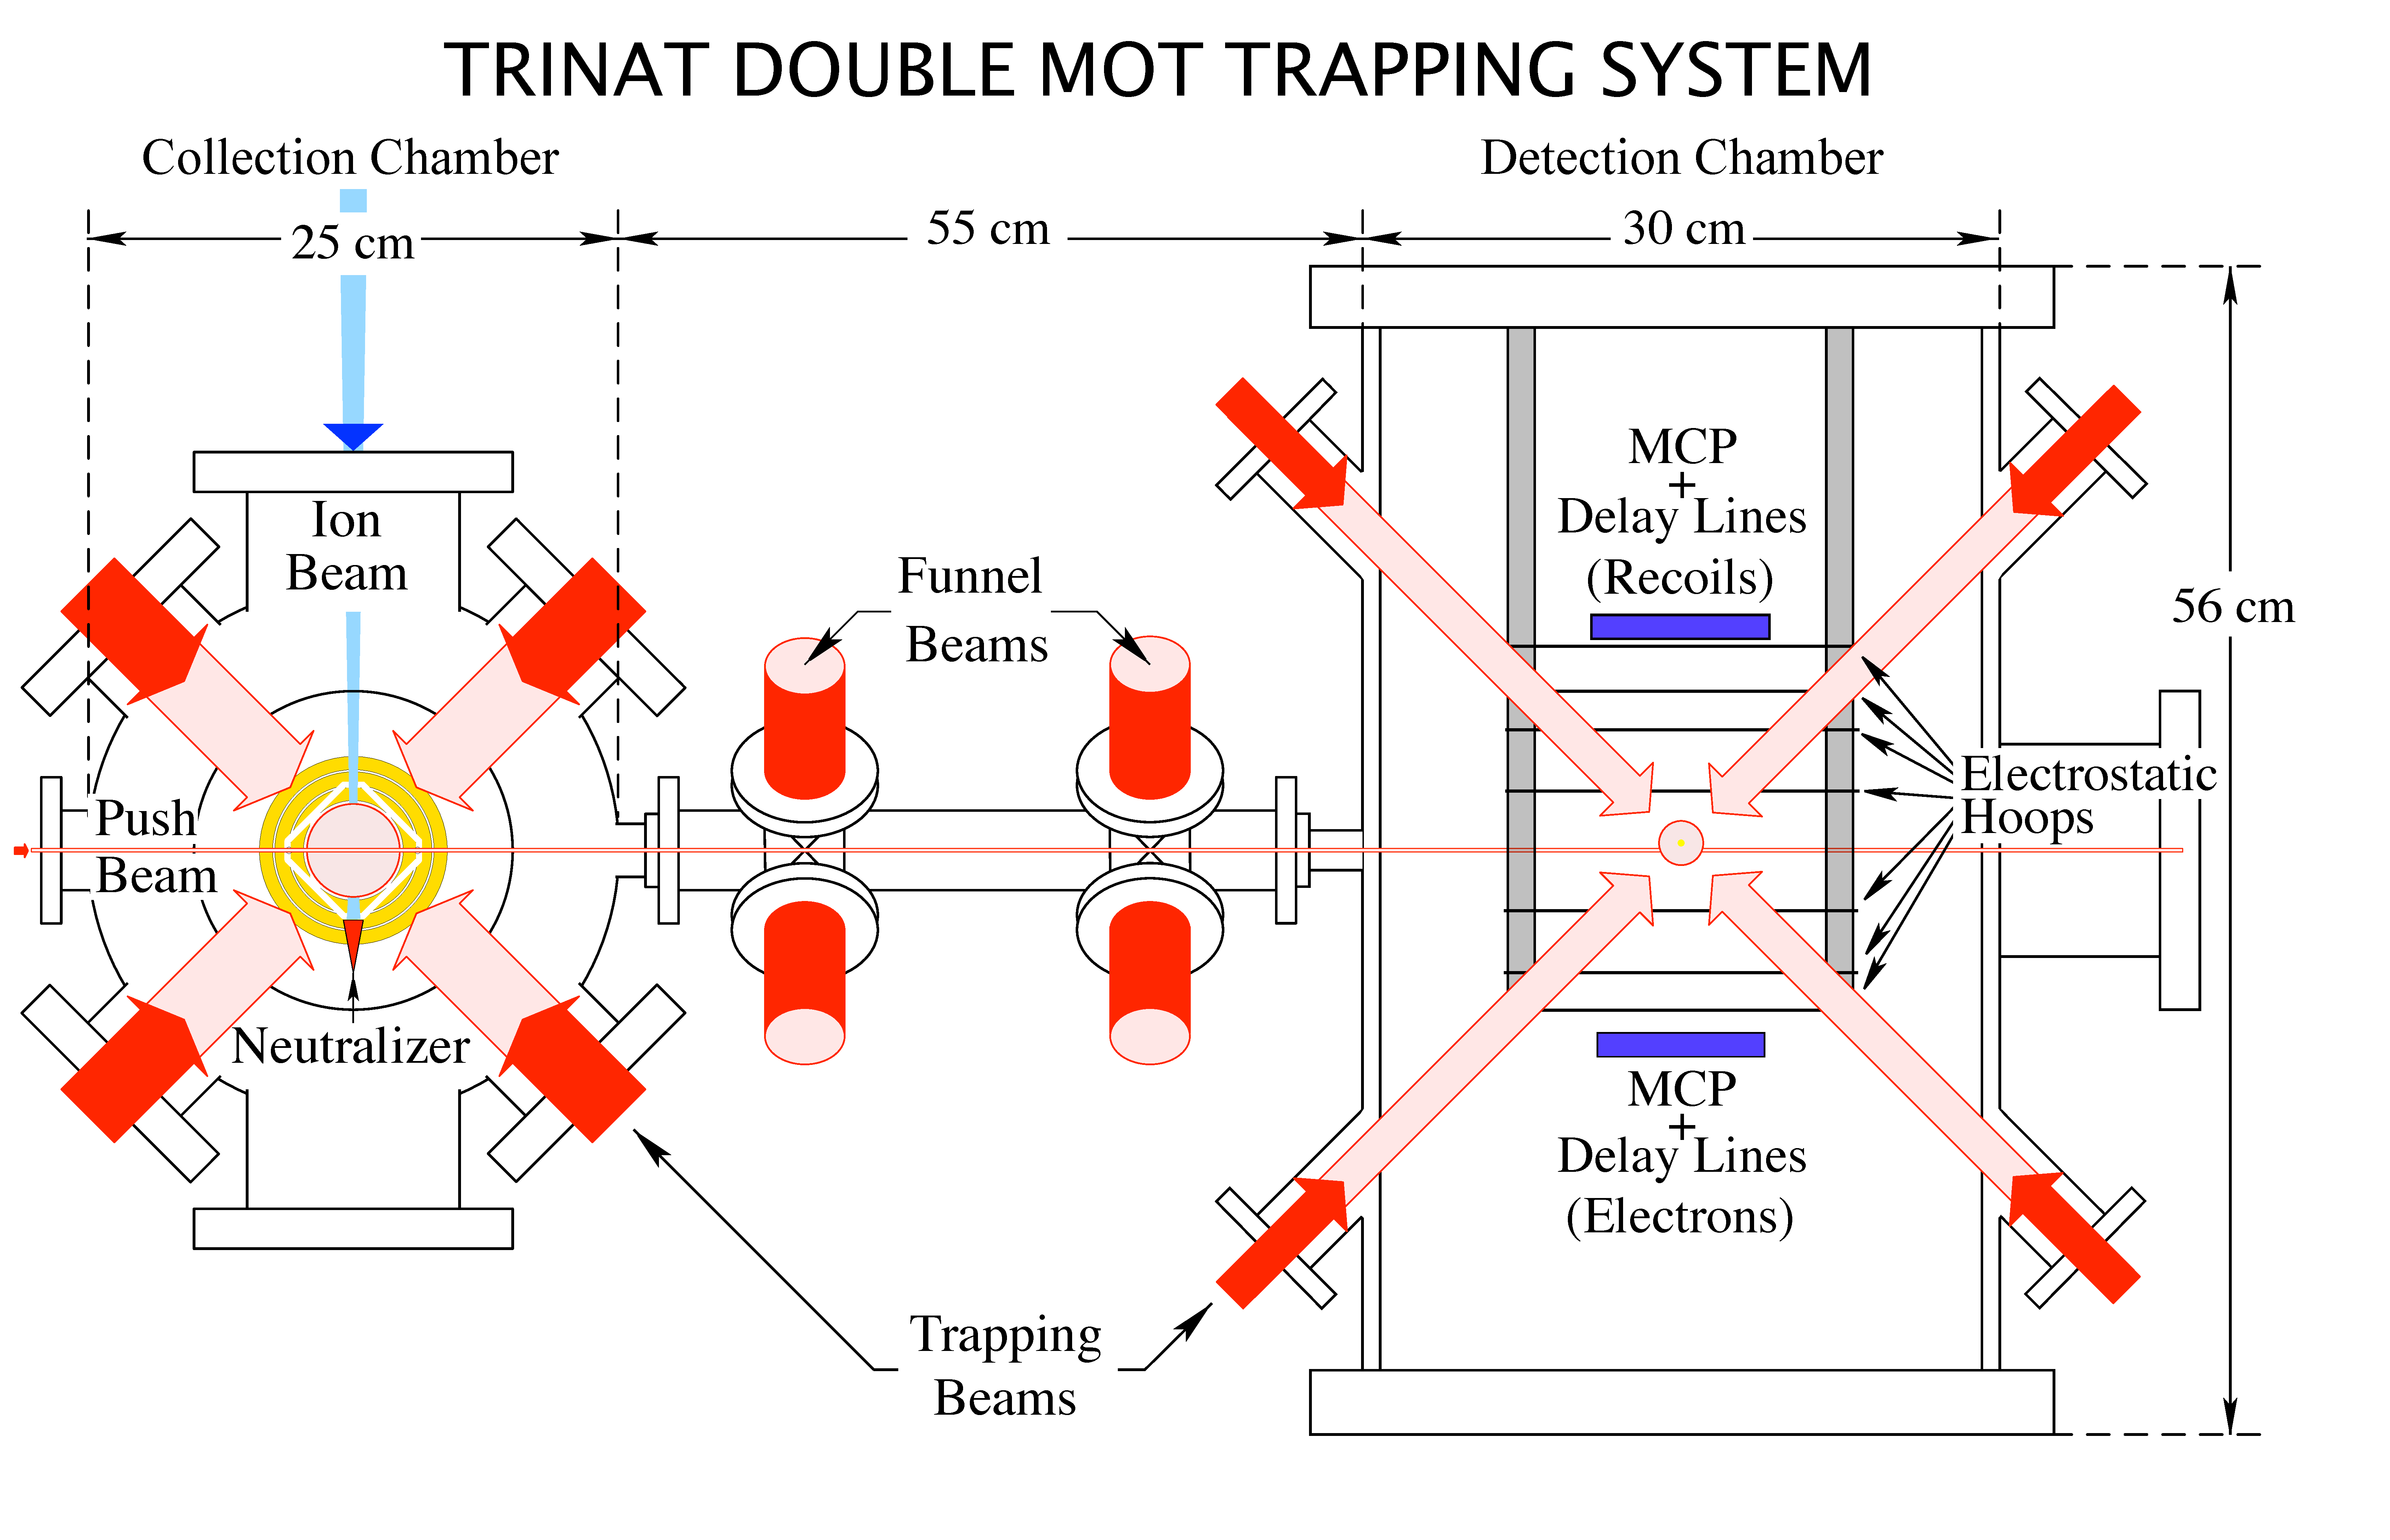
\includegraphics[width=.999\linewidth]
	{Figures/doublemot4.pdf}
	\caption{The TRINAT experimental set-up, viewed from above.  The two MOT system reduces background in the detection chamber.  Funnel beams along the atom transfer path keep the atoms focused.}	
	\label{fig:doublemot}
\note{Figure was originally created by Alexandre, modified by ... someone else?  Or Alexandre?  And I got it from ... probably an experimental proposal?  I should figure out how to cite a proposal...}
\end{figure}

The TRINAT lab accepts radioactive ions delivered by the ISAC beamline at TRIUMF.  These ions are collected on the surface of a hot zirconium foil where they are electrically neutralized, and subsequently escape from the foil into the first of two experimental chambers (the ``collection chamber").  Further details on the neutralization process are presented in a previous publication~\cite{gorelov2000}.  Within the collection chamber, atoms of one specific isotope -- for the purposes of this thesis,  \isotope[37]{K} -- are continuously collected into a magneto-optical trap 
%(MOT)\aside[color=org]{defined `MOT' in Ch.3.} 
from the tail end of the thermal distribution.  Although this procedure preferrentially traps only the slowest atoms, once trapped, atoms will be cooled further as a side-effect of the MOT's trapping mechanism.  The result is a small ($\sim\!1\,$mm diameter), cold ($\sim\!1\,$mK) cloud of atoms of a particular isotope.  
\note{Mumble mumble UHV.  Mumble mumble tail end of the Boltzmann distribution.}

These properties of the atomic cloud allow for a relatively clean transfer of linear momentum from an appropriately tuned laser beam to the atoms within the cloud, and we use this mechanism to ``push'' the atoms out of the collection MOT and into the ``detection chamber'', where they are loaded into a second MOT (see Fig.~\ref{fig:doublemot}).  During regular operation, atoms are transferred approximately once per second.  

There is no need to release previously trapped atoms in the second MOT when a new group of atoms is loaded.  Although the trap loses atoms over time as a result of a variety of physical processes,\aside{discussed ... idk, somewhere else.} during typical operation the majority of atoms loaded in a given transfer will still be trapped at the time the next set of atoms is loaded, and after several transfer cycles, something like a steady state is obtained.

%It should be noted that this loading process does not require atoms already trapped within the second MOT to be released when the next set of atoms is loaded.  Although there are several loss mechanisms 

Because the transfer and trapping mechanisms rely on tuning laser frequencies to specific atomic resonances, these mechanisms act on only a single isotope, and all others remain unaffected.  The result is a significant reduction of background contaminants within the detection chamber relative to initial beamline output.  The transfer methodology is discussed in some detail within another publication~\cite{swanson}.

%this setup allows for the selection of only a single isotope within the detection MOT, and a significantly reduced background relative to the initial beamline output. 

%\note{Probably describe the laser transfer method slightly.}  

%The TRIUMF Neutral Atom Trap (TRINAT) offers an experimental set-up which is uniquely suited to precision tests of Standard Model beta decay physics.  Radioactive ions are delivered from the ISAC beamline and neutralized before being trapped in the first of two magneto-optical traps (MOTs).  Approximately once per second, atoms from the first MOT are transferred to the second, where their decay products can be observed with significantly less background than would have been possible in the first trap (see Figure~\ref{fig:doublemot}).  The transfer methodology is discussed in some detail in a paper by Swanson et al~\cite{swanson}. \aside{The point is that this eliminates background from the decays of other stuff.  Or the same stuff.  Stuff that's not centered at the trap.}

We now turn our attention to what happens to the atom cloud in the detection chamber between loading phases (see Fig.~\ref{fig:dutycycle}).  One of the goals for the 2014 $^{37}\textrm{K}$ beamtime required that the atom cloud must be spin-polarized, as well as being cold and spatially confined.  Although the MOT makes it straightforward to produce a cold and well confined cloud of atoms, it is fundamentally incompatible with techniques to polarize these atoms. The physical reasons behind this are discussed in Section~\ref{section:acmot_and_polarization}.~\aside[color=org]{I *do* discuss this, right?  Right??}
% One goal for the 2014 $^{37}\textrm{K}$ beamtime was to perform a precision measurement of the beta asymmetry, 

\begin{figure}[h!!]
	\centering
	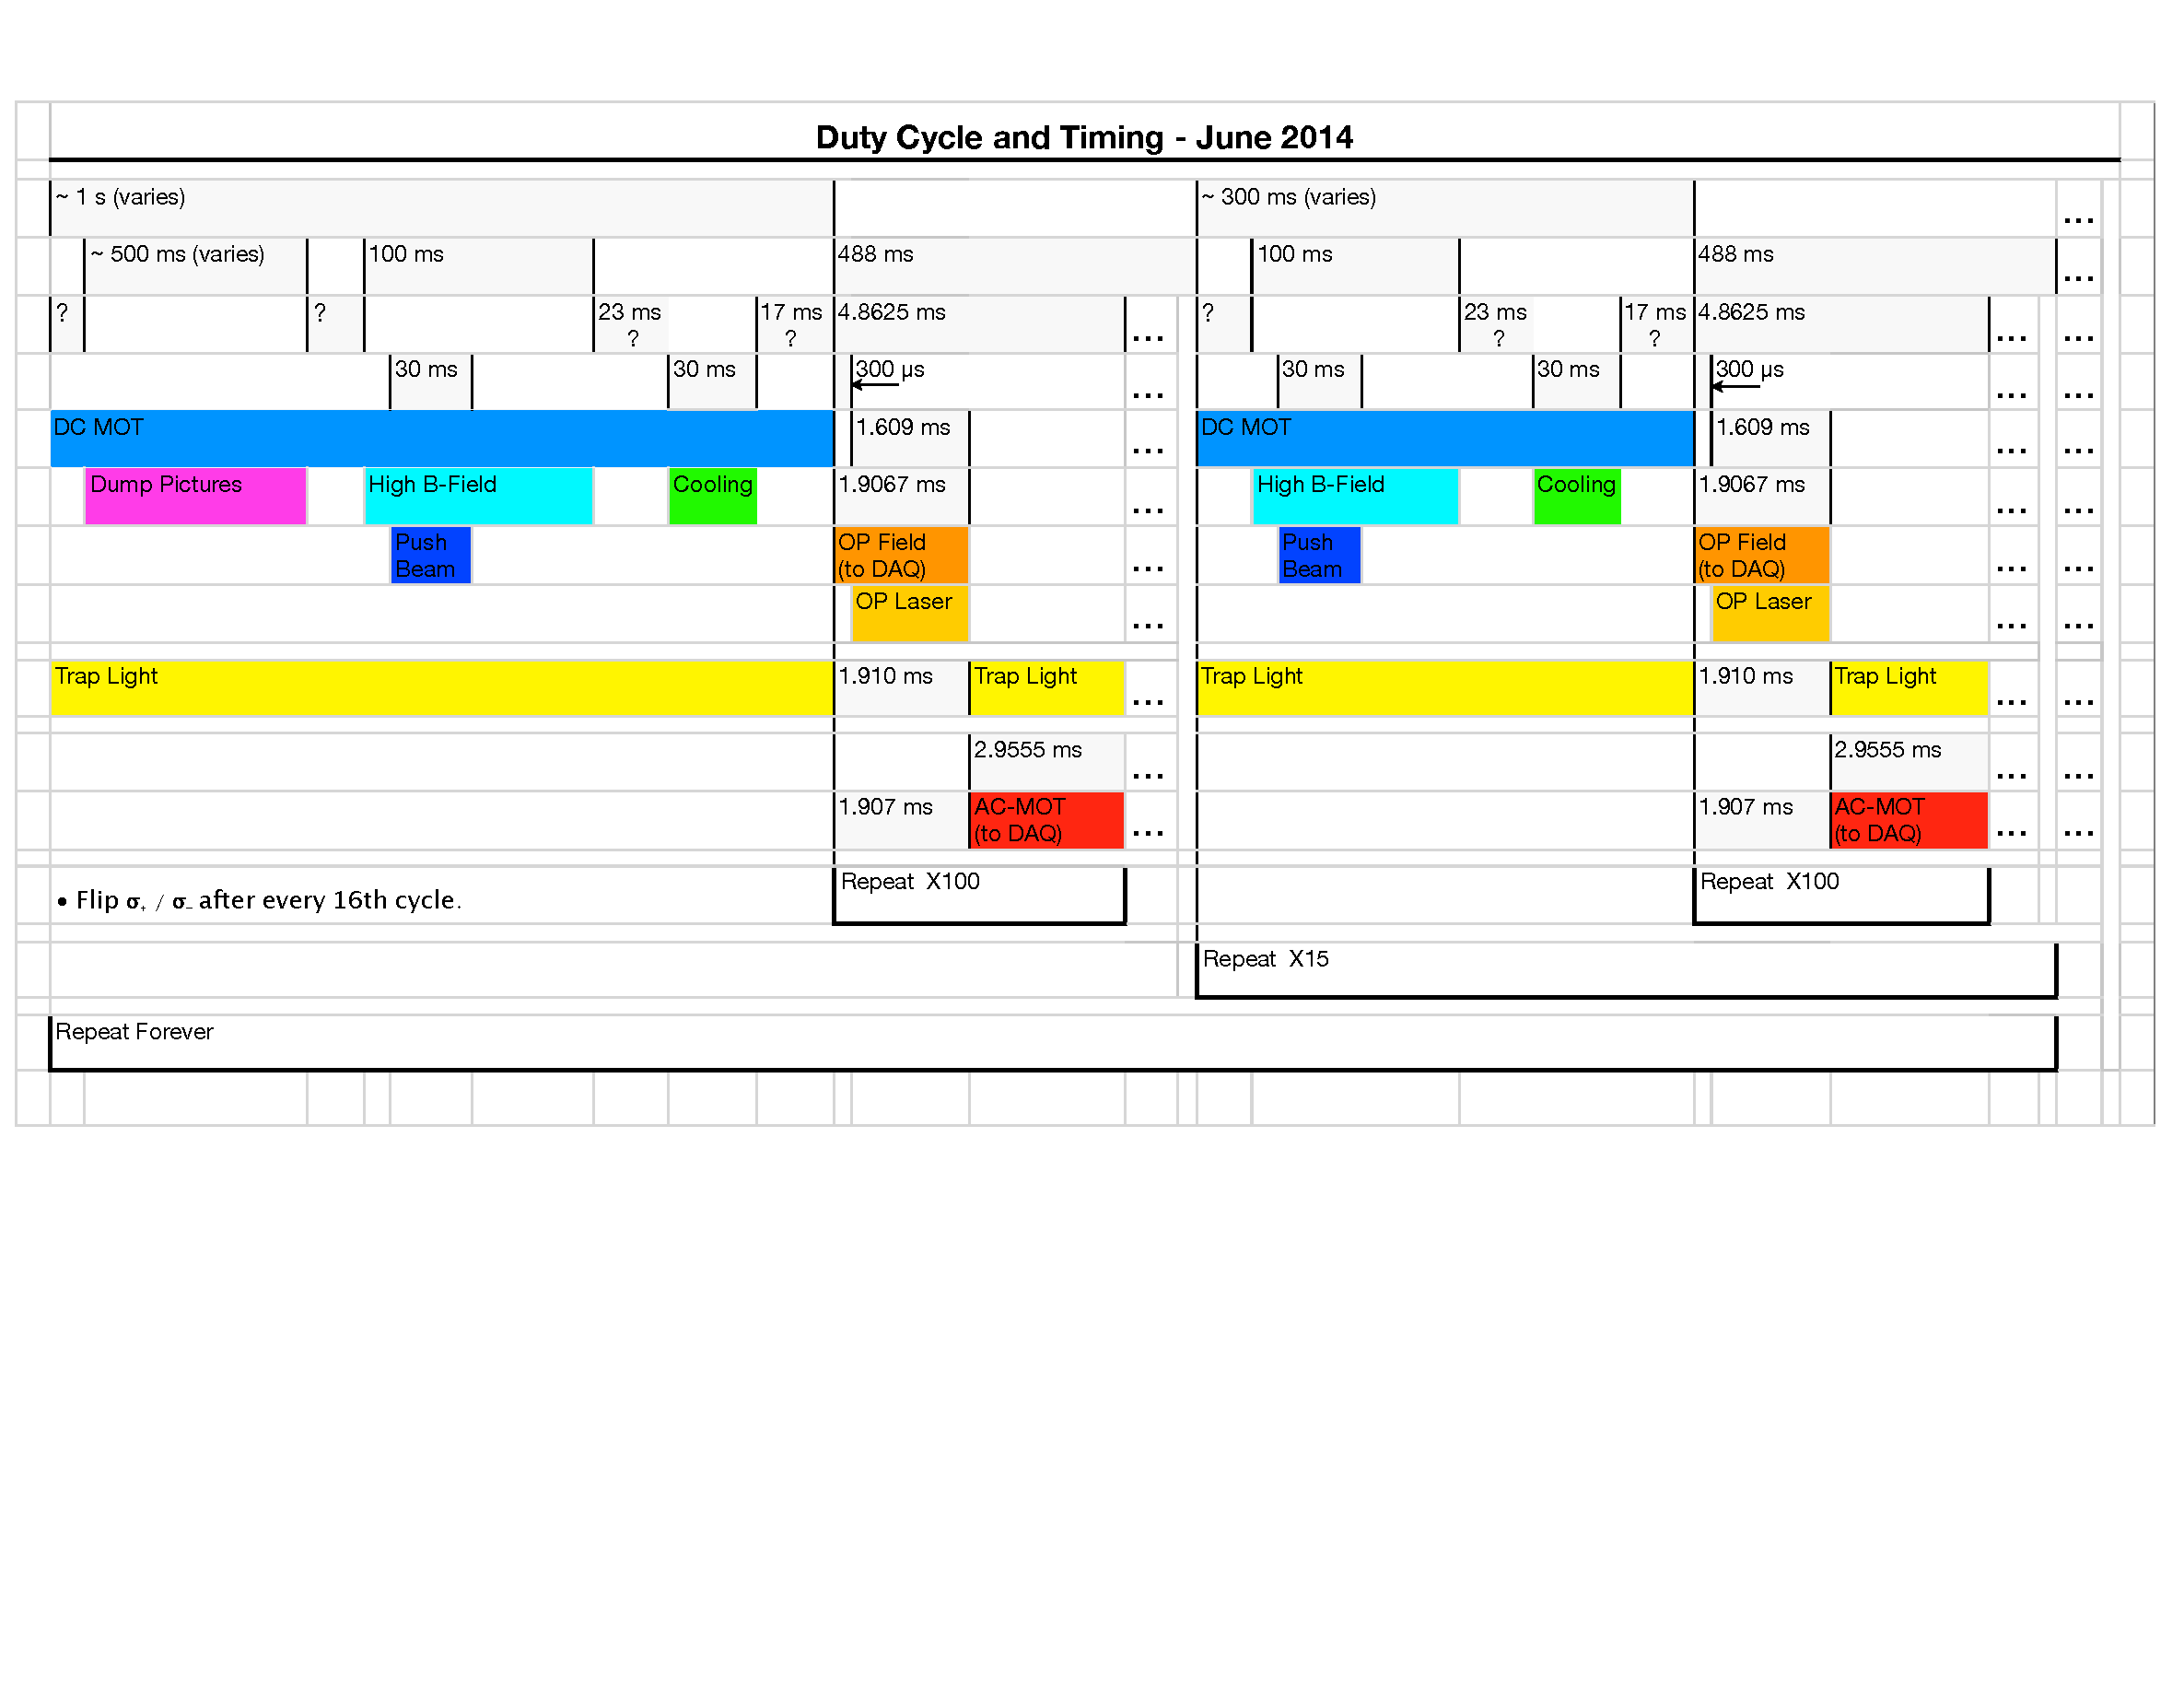
\includegraphics[width=.999\linewidth]
	{Figures/DutyCycle_2014.pdf}
	\caption{The duty cycle used for transferring, cooling, trapping, and optically pumping $\isotope[37]{K}$ during the June 2014 experiment.  Not drawn to scale.  Question marks indicate timings that varied either as a result of electronic jitter or as a result of variable times to execute the control code.  Atoms are transferred during operation of the DC-MOT.  Though the push beam laser itself is only on for $30\,$ms, the bulk of the DC-MOT's operation time afterwards is needed to collect and cool the transferred atoms.  After 100 on/off cycles of optical pumping and the AC-MOT, the DC-MOT resumes and the next group of atoms is transferred in.  After 16 atom transfers, the polarization of the optical pumping laser is flipped to spin-polarize the atoms in the opposite direction, in order to minimize systematic errors.}	
	\label{fig:dutycycle}
\end{figure}

Once the newly transferred set of $^{37}\textrm{K}$ atoms has been collected into the cloud, the entire MOT apparatus cycles 100 times between a state where it is `on' and actively confining atoms, and a state where it is `off' and instead the atoms are spin-polarized by optical pumping while the atom cloud expands ballistically before being re-trapped.  These 100 on/off cycles take a combined total of $488\,$ms.  The laser components of the trap are straightforward to cycle on and off on these timescales, but the magnetic field is much more challenging to cycle in this manner.  

\note[color=org]{How to segue here?  Do I...  Cite myself?  Cite Harvey+Murray?  Reference the next section?  Reference the previous chapter?  This is clunky and stupid.}
%Once the newly transferred atoms have arrived at the second trap, the MOT cycles 100 times between a state where it is `on' and actively confining atoms to a region of approximately 2\,mm$^3$, to a state where it is `off' and instead the atoms are spin-polarized by optical pumping while the atom cloud expands ballistically before being re-trapped.  
Immediately following each set of 100 optical pumping cycles, another set of atoms is transferred in from the collection chamber to the detection chamber, joining the atoms that remain in the trap (see Fig.~\ref{fig:dutycycle}).  The details of the trapping and optical pumping cycles are described further in Section~\ref{section:acmot_and_polarization}, and the optical pumping technique and its results for this beamtime are the subject of a recent publication~\cite{ben_OP}.



%%% % % % %%%
\section{The AC-MOT and Polarization Setup}
%\subsection{The AC-MOT}
\label{sec:acmot}
\label{section:acmot_and_polarization}

%\note[color=org]{This section is probably redundant with Sec.~\ref{section:acmot_and_polarization}. Remove *this* section.}
\note[color=jb]{JB on Ch. 3.4 (now 2.4) ((now Ch.~\ref{sec:acmot})) ``The AC-MOT'' (that's this section!):
The content and scope are ok, but the informal phrasing is going to
confuse people. You have to pay some attention and rephrase these sections.}
\note[color=jb]{John suggests that maybe I should just refer directly to his red, quoted OP blurb in the chapter about the AC-MOT.}

%\note[color=jb]{John suggests that maybe I should just refer directly to Sec.~\ref{photoions} in the chapter about the AC-MOT..}
%\note[color=jb]{``...Then you can refer to that(ie, Sec.~\ref{photoions}) in section 3.4 (now 2.4, about the AC-MOT, which is here.), where you're trying to now but the phrasing is poor.''}


Citation for Harvey and Murray goes here~\cite{harveymurray}.  Also, myself~\cite{thesis}.
%\note[color=jb]{``...where you're trying to now but the phrasing is poor.''}

%\note{Needs work.}

Here's a diagram of our AC-MOT running one AC-MOT/OP cycle, in Fig.~\ref{fig:acmot}.

\begin{figure}[ht]
	\centering
		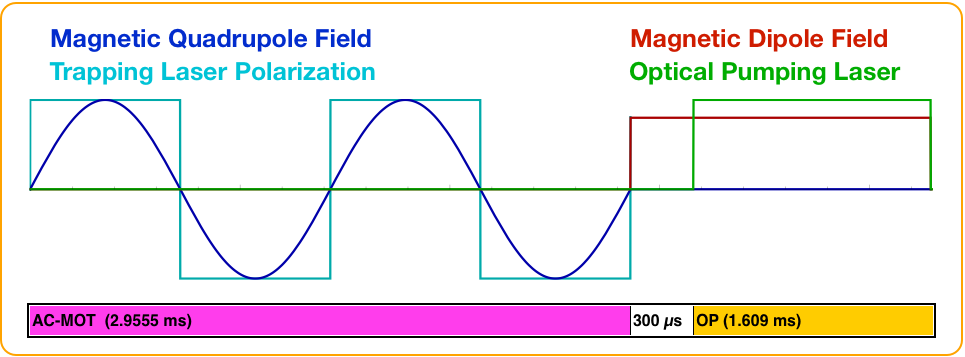
\includegraphics[width=.999\linewidth]{acmot.png}
		\caption{One cycle of trapping with the AC-MOT, followed by optical pumping to spin-polarize the atoms.  After atoms are transferred into the science chamber, this cycle is repeated 100 times before the next transfer.  The magnetic dipole field is created by running parallel (rather than anti-parallel as is needed for the MOT) currents through the two coils.}
		\label{fig:acmot}
\end{figure}


Normal MOTs are DC-MOTs.  They just sort-of go.  It's continuous.  We used an AC-MOT though!  The point of an AC-MOT is to shut off the magnetic field as quickly as possible.  With a well-controlled and uniform magnetic field, we can optically pump the atoms, which I think I'm going to describe in the upcoming section~(\ref{sec:op}).

Sadly, this also removes our trapping mechanism.  We could keep the optical molasses after the field is off if we wanted to, but we don't, because we wouldn't be able to optically pump the atoms then.  But at least the atoms are cold-ish (we can measure!  I think it's done indirectly in that one table, or for realsies in Ben's thesis), so we can let them just chill for a little while before we have to re-trap them.  Don't lose too much.  \aside{How much do we lose?  Have we quantified that somewhere?  Probably.}

Anyway, the idea of the AC-MOT is to run a sinusoidal current through your anti-Helmholtz coils.  You'll get eddy currents in your nearby metal *stuff* when you have a changing current, and those will *also* make a magnetic field. So, the idea with an AC-MOT is that with a sinusoid, you have clear control over what the eddy currents are actually doing, and you can just shut the current off when the eddy currents are zero (current in the anti-Helmholtz coils will be close to zero at this time too, depending on frequency of the sinusoid...), so you can reduce the size of the eddy currents by like an order of magnitude.  Eddy currents in general take a while to die away, so it's good to make them as small as possible.  ...Also, eddy currents making a magnetic field will screw up your optical pumping, because .... um, reasons?  I think it's not just the detuning, it's also something about the Larmor precession.  

%	
%	
%%%% --- * --- %%%%	
%%\subsection{The AC-MOT and Polarization Setup}
%\note[color=org]{This section is probably redundant with Sec.~\ref{sec:acmot}. Remove *that* section, keep this one.}
\note{begin content of the historical other AC-MOT+Polarization section.}
%\note[color=jb]{JB on Chapter 4.2 "The AC-MOT and Polarization Setup" (that's this section!):
%\\...\\
%"We use only the polarized portion of the duty cycle in
%order to minimize other systematic errors, such as the scintillator energy calibration
%and overall trap position."
%\\ ... \\
%We need to fix this. We use the polarized portion of the cycle because the
%atoms are almost totally polarized during it, and almost totally unpolarized
%outside of it. You leave the impression we could measure bFierz during the
%rest of the cycle, during unpolarized time ? 
%\\ ... \\
%MJA:  Ugh, no, that's really not what I meant.  Oh well, time to rephrase.}
%\\*

\note{Probably document things about the waveform and frequency used for the beamtime, since I don't think it's in my MSc.}

%\note[color=org]{Some of the contents of this section should be removed from here and moved over to Ch-3.  Probably.}

% 
\note[color=jb]{John objects to the phrasing of the following paragraph, because you fundamentally need polarized atoms to measure $\bFierz$.}
% Below:  John objects to this phrasing.  Admittedly, it gives the wrong impression. 
As alluded to in the previous section~(\ref{section:overview}), the measurement in question required a spin-polarized sample of atoms, and a precise knowledge of what that polarization was.  This was primarily needed in order to facilitate a measurement of $A_{\mathrm{\beta}}$ 
%\aside[color=org]{have I defined the beta asymmetry yet in some previous chapter?  otherwise I have to do it here..} 
that was performed on the same data that is the subject of discussion here.~\cite{ben_Abeta}   
%In order to facilitate a measurement of $A_{\mathrm{\beta}}$, great efforts were taken to polarize the atom cloud, and to quantify that polarization.  
% %This resulted in a duty cycle in which the atoms were intermittently trapped in the AC-MOT, then optically pumped to polarize them.  
While this is arguably less critical to a measurement of $b_{\mathrm{Fierz}}$,
%\aside[color=org]{have I defined $b_{\mathrm{Fierz}}$ yet?} 
it can still be an asset for eliminating systematic effects.  \aside{Plus, it barely makes sense to talk about measuring $\bFierz$ if you don't know $\Abeta$.}  
We use only the polarized portion of the duty cycle in order to minimize other systematic errors, such as the scintillator energy calibration and overall trap position.  It also makes for a more straightforward interpretation of the relationship of the measured values of $\Abeta$ and $\bFierz$ when the systematic effects are the same for both measurements. Finally, using only polarized data allows us to make use of the `superratio' construction in data analysis, a powerful tool for reducing (many) systematic errors at the expense of statistical precision (see Chapter~\ref{signature_chapter}).
% 
%\note[color=org]{I could move this (above) whole paragraph over to Ch.5 ((ch.4?)), where I surely discuss this in more detail.  It provides nice context here though.}
\note[color=jb]{End paragraph that John hates.}
%\note{In order to eliminate systematic effects, the polarization direction is flipped every 16 seconds.}
The Magneto-Optical Trap is a well-known technique from atomic physics, used to confine and cool neutral atoms~\cite{raabprentiss}, and it is also discussed in more detail in Chapter~\ref{atomicphysics_chapter}.
%\aside[color=org]{Should I move a bunch of this section's content over there, to live in Ch.3??  Should I move a bunch of content from Ch.3 to live here?  Current thinking:  It seems best to split the content up into a general picture of the MOT (Ch.3), and stuff that's unique to this experiment (here). }

%The technique is used predominantly with alkalis due to their simple orbital electron structure, so is appropriate for use with $^{37}\textrm{K}$.  Once set up, it is quite robust, and the trapping force is specific to the isotope for which the trap has been tuned. This feature makes it ideal for use in radioactive decay experiments, since the daughters are unaffected by the trapping forces keeping the parent confined.
%\note[color=org]{I think most of the above paragraph is also written/paraphrased elsewhere.  eg, the chapter on MOTs in general, and the previous section describing our 2-MOT system.  Do I need to move things around?}

%There are two primary components necessary for any MOT:  a laser, and a magnetic field.  The laser, which must be circularly polarized in the appropriate directions and tuned slightly to the red of an atomic resonance, is split into three perpendicular retroreflected beams, doppler cooling the atoms and (with the appropriate magnetic field) confining them in all three dimensions (see Figure~\ref{fig:mot}).  
%\note{Removed:  stuff about how a MOT works.  It's in Ch.3 ((Ch.2 now.  That's *basically* here.))  It lives there now.}
The TRINAT science chamber includes 6 `viewports' specifically designed to be used for the trapping laser (see Fig.~\ref{fig:thechamber}.).

%\missingfigure{This is going to need another edge-on G4 picture of the chamber to label all the atomic components.  }
%\[\]

%\note{Is my photoionization description adequate?  ... in light of John's feedback:  no.}
\note[color=jb]{JB says:  ``Since you worked hard on the logic triggers, a photoion spectrum with duty cycle would be appropriate if you want."}

%\note{Need to describe how polarization works.}
%\note[color=jb]{JB says:  all polarization details could be deferred to ~\cite{ben_OP}.  (be sure to list all authors including [me]).  )}

A MOT also requires a quadrupolar magnetic field, which we generate with two current-carrying anti-Helmholtz coils located within the vacuum chamber itself.  The coils themselves are hollow, and are cooled continuously by pumping temperature-controlled water through them.   

One feature which makes our MOT unusual has been developed as a result of our need to rapidly cycle the MOT on and off -- that is, it is an ``AC-MOT''.  Rather than running the trap with one particular magnetic field and one set of laser polarizations to match, we run a sinusoidal AC current in the magnetic field coils, and so the sign and magnitude of the magnetic field alternate smoothly between two extrema, and the trapping laser polarizations are rapidly swapped to remain in sync with the field~\cite{harveymurray}\cite{thesis}.  See Figure~\ref{fig:acmot}.  

\note{Note that because the atoms within a MOT can be treated as following a thermal distribution, some fraction of the fastest atoms continuously escape from the trap's potential well.  Even with the most carefully-tuned apparatus, the AC-MOT cannot quite match a similar standard MOT in terms of retaining atoms.  The TRINAT AC-MOT has a `trapping half-life' of around 6 seconds, and although that may not be particularly impressive by the standards of other MOTs, it is more than adequate for our purposes.  $^{37}\textrm{K}$ itself has a radioactive half-life of only 1.6 seconds 
(cite someone), so our dominant loss mechanism is radioactive decay rather than thermal escape. }


%\note[color=lgrey]{Anyway, here's some figures.  Or possibly one figure.  Whatever.  Also, here's a reference to a figure.  See Fig.~\ref*{fig:themot} (works -- currently ``3.4"), or also its subfigures, eg Fig.~\ref{fig:acmot} (works -- currently ``3.4b") and Fig.~\ref{fig:mot} (works -- currently ``3.4a").  Maybe I have to subref them?  Like, eg, Subfig.~\subref{fig:acmot} (works -- currently ``3.4b") and Subfig.~\subref*{fig:mot} (works -- currently ``3.4a").  What if we try to subref everything?  Consider, eg, Fig.~\subref{fig:themot} (doesn't work).  Yeah, ok, so fortunately the note cites like the text.  This gives an example of shit to do and not to do.  Also, can't do a linebreak within a note.}  

%% !TEX root = ../thesis_main.tex

% fig:themot
% 	fig:mot
% 	fig:acmot

\begin{figure}[ht]
	\centering
	\begin{subfigure}[t]{0.242\textwidth}
		\centering
		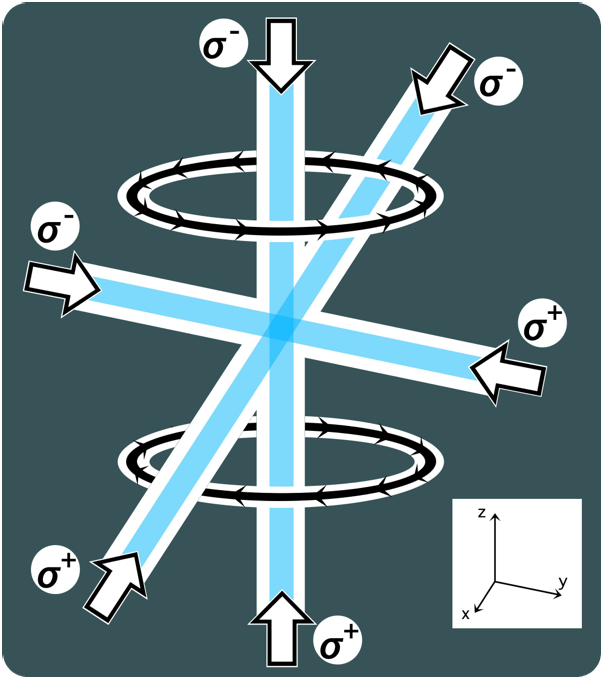
\includegraphics[width=\textwidth]{mot.png}
		\caption{Components of a magneto-optical trap, including current-carrying magnetic field coils and counterpropagating circularly polarized laser beams.}
		\label{fig:mot}
	\end{subfigure}
	\hfill
	\begin{subfigure}[t]{0.728\textwidth}
		\centering
		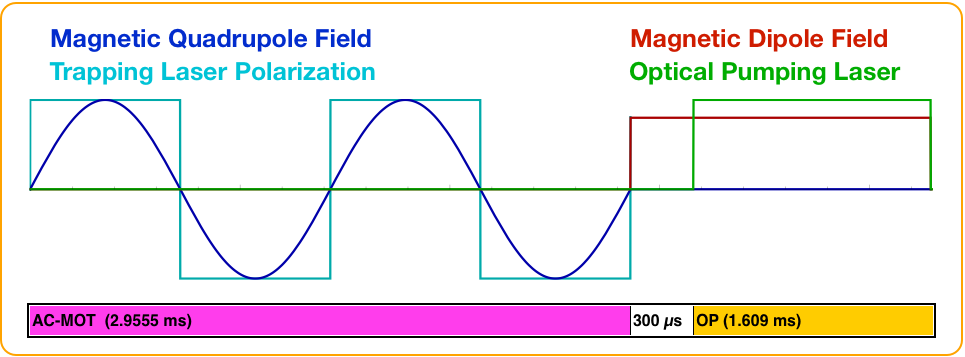
\includegraphics[width=\textwidth]{acmot.png}
		\caption{One cycle of trapping with the AC-MOT, followed by optical pumping to spin-polarize the atoms.  After atoms are transferred into the science chamber, this cycle is repeated 500 times before the next transfer.  The magnetic dipole field is created by running parallel (rather than anti-parallel as is needed for the MOT) currents through the two coils.}
		\label{fig:acmot}
	\end{subfigure}
	\caption{An alternating-current magneto-optical trap with a duty cycle optimized for producing polarized atoms}	
	\label{fig:themot}
\end{figure}


%\begin{figure}[ht]
%	\centering
%		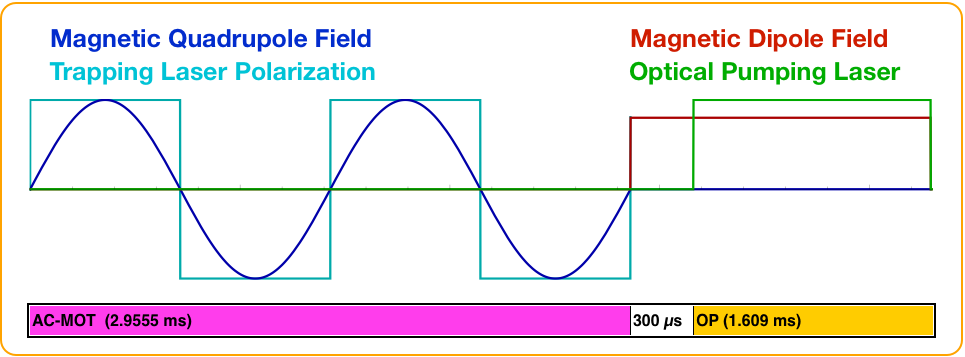
\includegraphics[width=.999\linewidth]{acmot.png}
%		\caption{One cycle of trapping with the AC-MOT, followed by optical pumping to spin-polarize the atoms.  After atoms are transferred into the science chamber, this cycle is repeated 100 times before the next transfer.  The magnetic dipole field is created by running parallel (rather than anti-parallel as is needed for the MOT) currents through the two coils.}
%		\label{fig:acmot}
%\end{figure}


We spin-polarize $^{37}\textrm{K}$ atoms within the trapping region by optical pumping~\cite{ben_OP}.  A circularly polarized laser is tuned to match the relevant atomic resonances, and is directed through the trapping region along the vertical axis in both directions.  When a photon is absorbed by an atom, the atom transitions to an excited state and its total angular momentum (electron spin + orbital + nuclear spin) along the vertical axis is incremented by one unit.  When the atom is de-excited a photon is emitted isotropically, 
%\comment{(is it still isotropic when it's polarized?  I bet it's not.)}
so it follows that if there are available states of higher and lower angular momentum, the \emph{average} change in the angular momentum projection is zero.  If the atom is not yet spin-polarized, it can absorb and re-emit another photon, following a biased random walk towards complete polarization.  

%\missingfigure{Need a picture of the whole duty cycle.  Possibly combine with ~\ref{fig:acmot}.}


In order to optimally polarize a sample of atoms by this method, it is necessary to have precise control over the magnetic field.  This is because absent other forces, a spin will undergo Larmor precession about the magnetic field lines.  In particular, the magnetic field must be aligned along the polarization axis (otherwise the tendency will be to actually depolarize the atoms), and it must be uniform in magnitude over the region of interest (otherwise its divergencelessness will result in the field also having a non-uniform direction, which results in a spatially-dependent depolarization mechanism).  Note that this type of magnetic field is not compatible with the MOT, which requires a linear magnetic field gradient in all directions (characteristic of a quadrupolar field shape), and has necessitated our use of the AC-MOT as described in (Sub-)Section~\ref{sec:acmot}. \aside[color=org]{At some point I have to decide if that's going to be a section or a subsection.}
%\aside{that's this section.  I should really describe the AC-MOT.}



%\section{Microchannel Plates and Electric Field}

%\color{black}
%	\subsection{\textbf{Nuclear Setup}}
\section{Measurement Geometry and Detectors}
\label{section:betadetectors}
\label{section:mcps}
\label{sec:geometry}
\note[color=jb]{JB says of ((Sec.~\ref{sec:geometry})):  first few paragraphs are poorly phrased. You have to fix those.  Most of the rest looks really good.  }
\note{This section is really disorganized.}
\note{Possibly needs more diagrams?  Possibly just needs more words.}

MCPs.  Hoops.  Only one MCP works at a time!  Blarg.  Upon decay, atoms literally aren't trapped anymore by the trap.  No trapping forces, no slowing forces, because it's all isotope-specific.

Back-to-back MCPs in an electric field to tag events from the trap, and to measure the trap position and polarization.  Hoops to produce the electric field.  The electric field sucks negatively charged electrons into one MCP, and positively charged ions into the other.  See Fig.~\ref{chamber_decayevent}

Back-to-back beta detectors along the polarization axis.  

%\comment{
  %Back-to-back beta detectors along the polarization axis.  Back-to-back MCPs in an electric field to tag events from the trap, and to measure the trap position and polarization.  Hoops to produce the electric field.  
	Many laser ports to make the MOT functional, and for optical pumping.  Fancy mirror geometry to combine optical pumping and trapping light along the vertical axis.  Water-cooled (anti-)Helmholz coils within the chamber for the AC-MOT, fast switching to produce an optical pumping field.  
%	\subsection{\textbf{All the Detectors}}
%}

%%%
\begin{figure}[h!!!!!t!!!!!]
	\centering
%	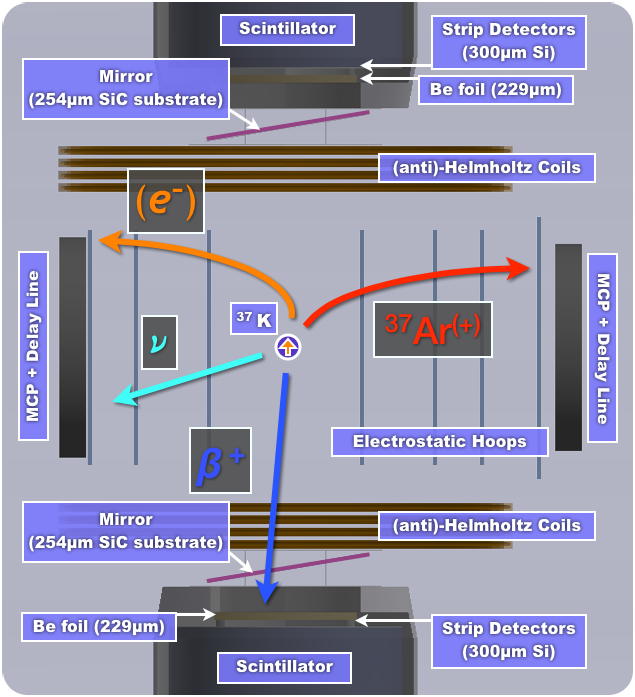
\includegraphics[width=.999\linewidth]{Figures/chamber_decayevent3.png}
	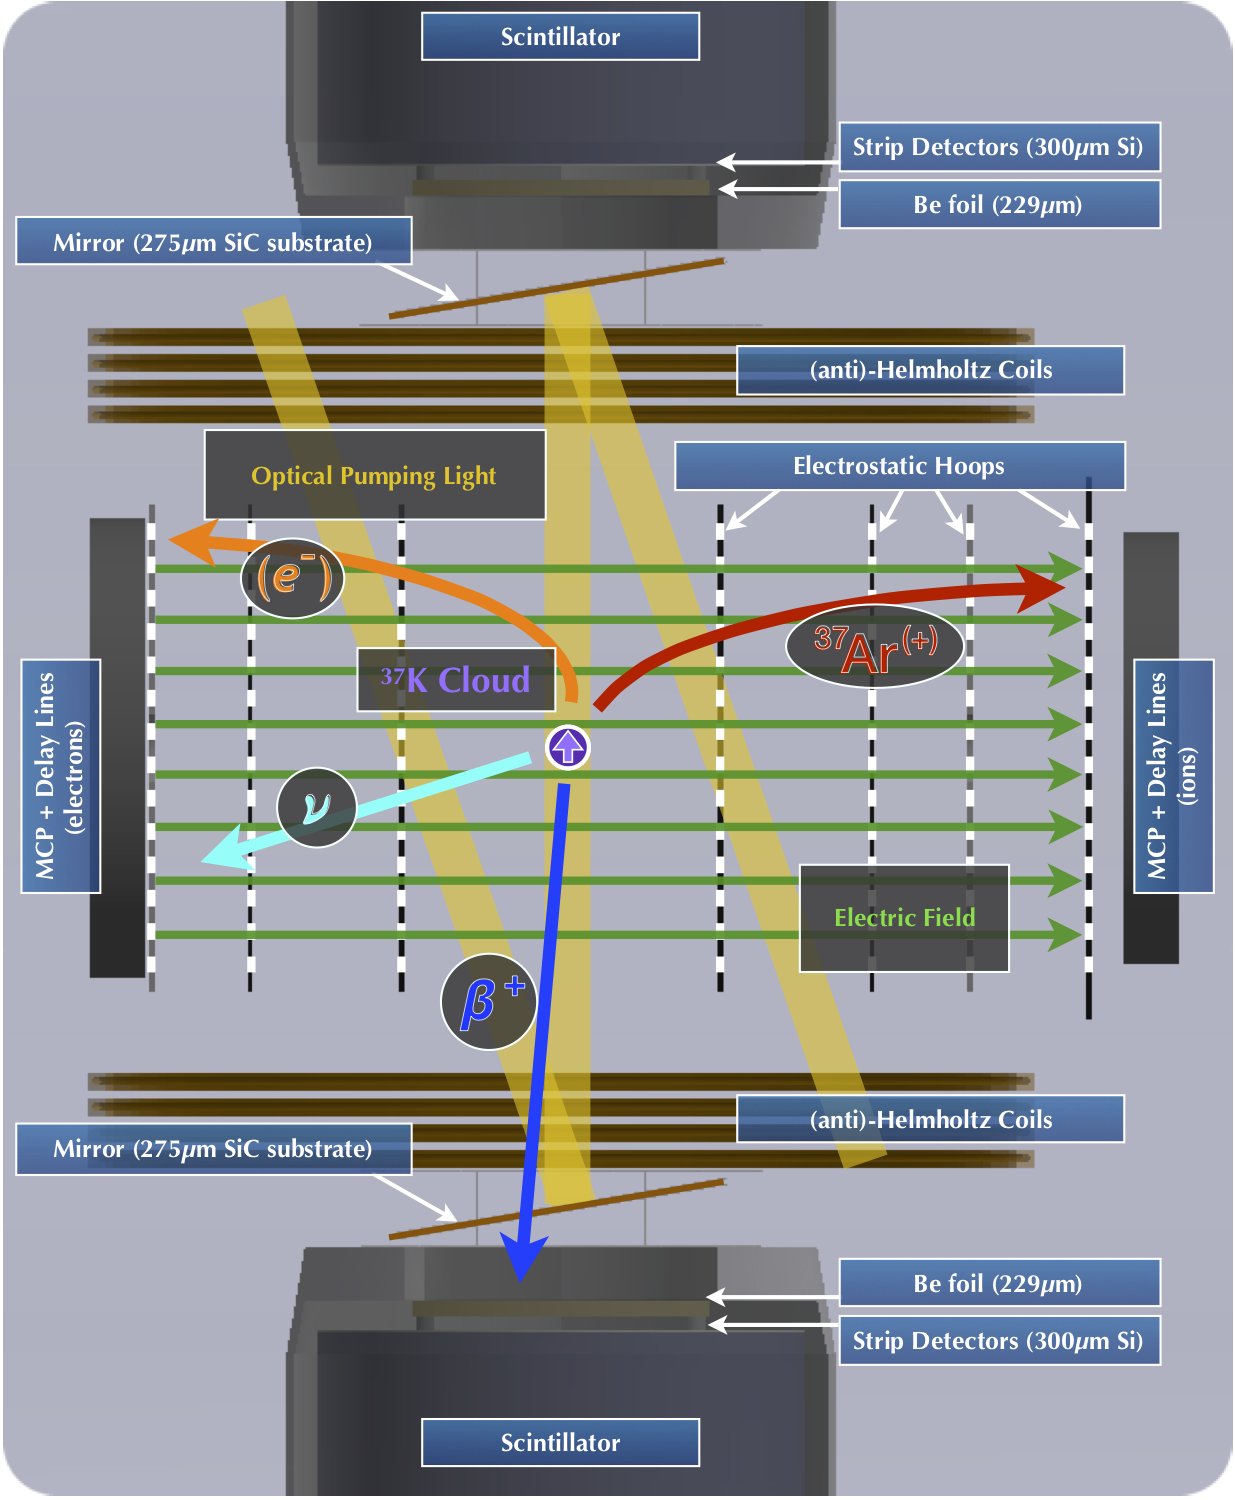
\includegraphics[width=.9\linewidth]{Figures/chamber_cross_section_with_event.png}
	\caption{A decay event within the TRINAT science chamber.  After a decay, the daughter will be unaffected by forces from the MOT.  Positively charged recoils and negatively charged shake-off electrons are pulled towards detectors in opposite directions.  Although the $\beta^+$ is charged, it is also highly relativistic and escapes the electric field with minimal perturbation.}
	%\comment{The pic is still kind-of fuzzy.}
%	\note{The pic is still kind-of fuzzy.}
%	\note{Mirrors are 275~$\mu$m thick, not the 254~$\mu$m shown in picture.}
%	\note{Must separate these pictures.  Probably also adjust (a) to show *all* the apparatus stuff, and make a separate one to show the decay.}
	\label{chamber_decayevent}
\end{figure}


%\note{Below is pretty vague.  I could do better, even for just an overview-summary thing.  Obvs I have to describe it in detail later on *somewhere*, though maybe not in the overview-summary...} 
Detectors are positioned about the second MOT for data collection.  The detection chamber 
%(shown in Figure \ref{fig:thechamber}) 
operates at ultra-high vacuum (UHV) and provides not only the apparatus necessary to intermittently confine and then spin-polarize atoms, but also the variety of detectors and implements required to quantify their position, temperature, and polarization.  The detection chamber further boasts an array of electrostatic hoops to collect both positively and negatively charged low energy particles into two microchannel plates (MCPs),  and a further set of two beta detectors positioned along the polarization axis, each of which consists of a 40x40 pixel double-sided silicon strip detector (DSSD) and a scintillator and photomultiplier tube (PMT).  %The details of the detection chamber setup are described in detail in Section~\ref{section:betadetectors}. 
%\note{ ...where I basically repeat this same content.  Blarg.}




\note{...(shown in Figure \ref{fig:thechamber}) ...}
The beta detectors, located above and below the atom cloud along the axis of polarization (see Figure~\ref{chamber_decayevent}), are each the combination of a plastic scintillator and a set of silicon strip detectors.  Using all of the available information, these detectors are able to reconstruct the energy of an incident beta, as well as its hit position, and provide a timestamp for the hit's arrival.  Together the upper and lower beta detectors subtend approximately 1.4\% of the total solid angle as measured with respect to the cloud position. 

%\section{Beta Detectors}
	The two sets of beta detectors were positioned directly along the axis of polarization.  Each beta detector consists of a plastic scintillator and photo-multiplier tube (PMT) \aside{There's gotta be a better way to describe it} placed directly behind a 40$\times$40-pixel double-sided silicon strip detector (DSSD).  \aside{what's the open area of the detector?  how big is each pixel?}  The scintillator is used to measure the overall energy of the incoming particles, as well as to assign a timestamp to these events, while the DSSD is used both to localize the hit position to one (or in some cases, two) individual pixel(s), and also to discriminate between different types of incoming particles.  In particular, though the scintillator will measure the energy of an incoming beta or an incoming gamma with similar efficiency, the beta will lose a portion of its kinetic energy as it passes through the DSSD into the scintillator.  By contrast, an incident gamma will deposit only a very small amount of energy in the DSSD layer, making it possible to reject events with insufficient energy deposited in the DSSD as likely gamma ray events.  Given that the decay of interest to us emits positrons, we expect a persistent background 511 keV gamma rays that are not of interest to us, so it is extremely important that we are able to clean these background events from our spectrum. 


It must be noted that the path between the cloud of trapped atoms and either beta detector is blocked by two objects:  a 275$\,\mu$m silicon carbide mirror (necessary for both trapping and optical pumping), and a 229$\,\mu$m beryllium foil (separating the UHV vacuum within the chamber from the outside world).  In order to minimize beta scattering and energy attenuation, these objects have had their materials selected to use the lightest nuclei with the desired material properties, and have been manufactured to be as thin as possible without compromising the experiment.  As the $^{37}\textrm{K} \rightarrow \,^{37}\textrm{\!Ar} + \beta^{+} + \nu_e$ decay proceess releases $Q=5.125$\,MeV of kinetic energy~\cite{Q_value}, the great majority of betas are energetic enough to punch through both obstacles without significant energy loss before being collected by the beta detectors.  

On opposing sides of the chamber, and perpendicular to the axis of polarization, two stacks of $\sim$ 80\,mm diameter microchannel plates (MCPs) have been placed (see Figure~\ref{fig:thechamber}) as detectors, providing a time stamp when a particle is incident on their surfaces.  Behind each stack of MCPs there is a set of delay lines, which provide  position sensitivity for these detectors.   

In order to make best use of these MCPs, we create an electric field in order to draw positively charged particles into one MCP, while drawing negatively charged electrons into the other MCP.  Seven electrostatic hoops have been placed within the chamber (see Figure~\ref{fig:thechamber}), and are connected to a series of high voltage power supplies.  See Sections~\ref{photoions} and~\ref{pos_recoils} for a discussion of what sort of charged particles we expect to observe in these detectors and how they are created.  
\note[color=org]{Wait.  Am I repeating myself?}

Scientific data has been collected at field strengths of 66.7 V/cm, 150 V/cm, 395 V/cm, 415 V/cm, and 535 V/cm.  It should be noted that these field strengths are too low to significantly perturb any but the least energetic of the (positively charged) betas from the decay process, and these low energy betas would already have been unable to reach the upper and lower beta detectors due to interactions with materials in the SiC mirror and Be foil vacuum seal.  



%%%% --- * --- %%%%	
\section{The Photoionization Laser}
\label{cloud}
\label{photoions}
%\note[color=org]{Some of this stuff is in Ch.3 (now ch.2) (see Section~\ref{sec:photoprobe}) ((now removed)) and/or Ch.6 (now ch.5) ((ch.4?)) (see Section~\ref{sec:cloud_calibration}).  Some of it *should* be.}
\note[color=jb]{Chapter 4.4 (this section!  now 3.4) (((~\ref{photoions}))) is very good and complete, showing you understand what isneeded about photoionization. A good reason to omit 3.5 `photoionization as a aprobe' as I said above.}

In order to measure properties of the trapped $^{37}\textrm{K}$ cloud, a 10\,kHz pulsed laser at 355\,nm is directed towards the cloud.  These photons have sufficient energy to photoionize neutral $^{37}\textrm{K}$ from its excited atomic state, which is populated by the trapping laser when the MOT is active, releasing 0.77\,eV of kinetic energy, but do not interact with ground state $^{37}\textrm{K}$ atoms.  The laser is of sufficiently low intensity that only $\sim 1\%$ of excited state atoms are photoionized, so the technique is only very minimally destructive.
%The laser is of sufficiently low intensity that the great majority\aside[color=jb]{JB:  ``On order 1\% are photoionized."} of excited state atoms are \emph{not} photoionized, so the technique is only very minimally destructive.  
\note{Probably worth mentioning that we test this stuff offline on stable \isotope[41]{K}. }


Because an electric field has been applied within this region (see Section~\ref{field})\aside[color=jb]{JB:  ``you could reference the letter for the value of the field 150V/cm.''} the $^{37}\textrm{K}^+$ ions are immediately pulled into the detector on one side of the chamber, while the freed $e^-$ is pulled towards the detector on the opposite side of the chamber.  Because  $^{37}\textrm{K}^+$ is quite heavy relative to its initial energy, it can be treated as moving in a straight line directly to the detector, where its hit position on the microchannel plate is taken as a 2D projection of its position within the cloud.  Similarly, given a sufficient understanding of the electric field, the time difference between the laser pulse and the microchannel plate hit allows for a calculation of the ion's initial position along the third axis.  

\note{As a check:  the camera measurements for photons from de-excitation.  It's aimed 35 degrees from vertical, with its horizontal axis the same as ..... one of the other axes.  I think it's the TOF axis.  I can check this when my computer comes back.   Also, there's an unknown additional delay between some of our DAQ channels that can't be explained by accounting for cable lengths, so we really like having the check there.}
\note[color=jb]{JB says:  ``yes, camera x-axis is tof axis.''}


With this procedure, it is possible to produce a precise map of the cloud's position and size, both of which are necessary for the precision measurements of angular correlation parameters that are of interest to us here.  However, it also allows us to extract a third measurement:  the cloud's polarization.

The key to the polarization measurement is that only atoms in the excited atomic state can be photoionized via the 355 nm laser.  While the MOT runs, atoms are constantly being pushed around and excited by the trapping lasers, so this period of time provides a lot of information for characterizing the trap size and position.  When the MOT is shut off, the atoms quickly return to their ground states and are no longer photoionized until the optical pumping laser is turned on.  As described in Section~\ref{op}, and in greater detail in~\cite{ben_OP}, the optical pumping process involves repeatedly exciting atoms from their ground states until the atoms finally cannot absorb any further angular momentum and remain in their fully-polarized (ground) state until they are perturbed.  Therefore, there is a sharp spike in excited-state atoms (and therefore photoions) when the optical pumping begins, and none if %\aside[color=jb]{JB points out that this should be ``if", not ``once".} 
the cloud has been fully polarized.  The number of photoion events that occur once the sample has been maximally polarized, in comparison with the size and shape of the initial spike of photoions, provides a very precise characterization of the cloud's final polarization~\cite{ben_OP}.



%\begin{figure}[h!!]
%	\centering
%	\includegraphics[width=.999\linewidth]
%	{Figures/DutyCycle_2014.pdf}
%	\caption{The duty cycle used for transferring, cooling, trapping, and optically pumping $\isotope[37]{K}$ during the June 2014 experiment.  Not drawn to scale.  Question marks indicate timings that varied either as a result of electronic jitter or as a result of variable times to execute the control code.  Atoms are transferred during operation of the DC-MOT.  Though the push beam laser itself is only on for $30\,$ms, the bulk of the DC-MOT's operation time afterwards is needed to collect and cool the transferred atoms.  After 100 on/off cycles of optical pumping and the AC-MOT, the DC-MOT resumes and the next group of atoms is transferred in.  After 16 atom transfers, the polarization of the optical pumping laser is flipped to spin-polarize the atoms in the opposite direction, in order to minimize systematic errors.}	
%	\label{fig:dutycycle}
%\end{figure}


%% !TEX root = ../thesis_main.tex


% "fig:thechamber"

\begin{figure}[h!!!tb]
	\centering
%	\hspace*{\fill}%
	\subfloat[A decay event within the TRINAT science chamber.  After a decay, the daughter will be unaffected by forces from the MOT.  Positively charged recoils and negatively charged shake-off electrons are pulled towards detectors in opposite directions.  Although the $\beta^+$ is charged, it is also highly relativistic and escapes the electric field with minimal perturbation.
	%\comment{The pic is still kind-of fuzzy.}
	]
	{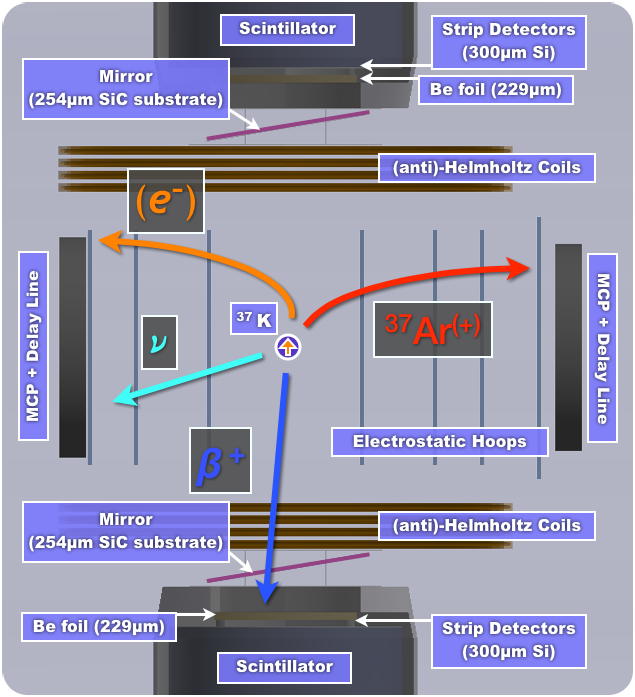
\includegraphics[width=.530\linewidth]{Figures/chamber_decayevent3.png}\label{chamber_decayevent} }
	\hspace*{\fill}
%	\hfill
	\hspace*{\fill}
	\subfloat[Inside the TRINAT science chamber.  This photo is taken from the vantage point of one of the microchannel plates, looking into the chamber towards the second microchannel plate.  The current-carrying copper Helmholtz coils and two beta telescopes are visible at the top and bottom.  The metallic piece near the center is one of the electrostatic `hoops' used to generate an electric field within the chamber.  The hoop's central circular hole allows access to the microchannel plate, and the two elongated holes on the sides allow the MOT's trapping lasers to pass unimpeded at an angle of 45 degress `out of the page'.]	
	{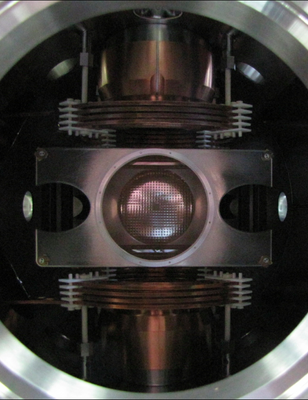
\includegraphics[width=.444\linewidth]{Figures/chamber_photo_2.png}}
%	\hspace*{\fill}%
	\caption{The TRINAT detection chamber}	
	\label{fig:thechamber}
\end{figure}


% "fig:thechamber"



%%%
\begin{figure}[h!!!tb]
	\centering
	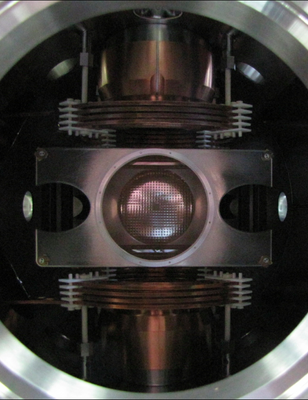
\includegraphics[width=.80\linewidth]{Figures/chamber_photo_2.png}
	\caption{Inside the TRINAT science chamber.  This photo is taken from the vantage point of one of the microchannel plates, looking into the chamber towards the second microchannel plate.  The current-carrying copper Helmholtz coils and two beta telescopes are visible at the top and bottom.  The metallic piece near the center is one of the electrostatic `hoops' used to generate an electric field within the chamber.  The hoop's central circular hole allows access to the microchannel plate, and the two elongated holes on the sides allow the MOT's trapping lasers to pass unimpeded at an angle of 45 degress `out of the page'.}
	\label{fig:thechamber}
\end{figure}



%%%% --- * --- %%%%	
%\section{Summary of Data Collected}
%
%\note[color=org]{Arguably I should put this stuff in Ch-6.  Maybe that's better...}
%\note{Really, this is missing a table.  At least one table.  I could probably justify putting in a few of them.
%\\...\\
%Things I could list:  Electric field strengths, eMCP/rMCP data type, triggers.  Photoions/Photoelectrons, betas, beta+electron/beta+recoil.  
%}




